        %%******************************************%%
        %%                                          %%
        %%        Modello di tesi di laurea         %%
        %%            di Andrea Giraldin            %%
        %%                                          %%
        %%             2 novembre 2012              %%
        %%                                          %%
        %%******************************************%%

\begin{document}
    \frontmatter
    \begin{titlepage}
    \begin{center}
        \begin{LARGE}
            \textbf{\myUni}\\
        \end{LARGE}

        \vspace{10pt}

        \begin{Large}
            \textsc{\myDepartment}\\
        \end{Large}

        \vspace{10pt}

        \begin{large}
            \textsc{\myFaculty}\\
        \end{large}

        \vspace{30pt}
        \begin{figure}[htbp]
            \centering
            
\includegraphics[height=6cm]{unipd-logo}
        \end{figure}
        \vspace{30pt}

        \begin{LARGE}
            \textbf{\myTitle}\\
        \end{LARGE}

        \vspace{10pt}

        \begin{large}
            \textsl{\myDegree}\\
        \end{large}

        \vspace{40pt}

        \begin{large}
            \begin{flushleft}
                \textit{Relatore}\\
                \vspace{5pt}
                \profTitle\ \myProf
            \end{flushleft}

            % You can tweak the spacing to have professor and student names on the same line
            % useful if the page is broken by a long thesis title and you need more space
            \vspace{-52pt}

            \begin{flushright}
                \textit{Laureando}\\
                \vspace{5pt}
                \myName
            \end{flushright}
        \end{large}

        \vspace{40pt}

        \line(1, 0){338} \\
        \begin{normalsize}
            \textsc{Anno Accademico \myAA}
        \end{normalsize}
    \end{center}
\end{titlepage}

    \clearpage
\phantomsection
\thispagestyle{empty}

\hfill
\vfill

\noindent\myName: \textit{\myTitle,}
\myDegree,
\textcopyright\ \myTime.

    \cleardoublepage
\phantomsection
\pdfbookmark{Ringraziamenti}{ringraziamenti}

\begingroup
\let\clearpage\relax
\let\cleardoublepage\relax
\let\cleardoublepage\relax

\chapter*{Ringraziamenti}

\noindent \textit{Innanzitutto, vorrei esprimere la mia gratitudine al Prof. \myProf, relatore della mia tesi, per l'aiuto e il sostegno fornitomi durante la stesura del lavoro.}\\

\noindent \textit{Ringrazio il mio tutor aziendale Roberto per avermi trasmesso con tenacia e passione le conoscenze del settore.}\\

\noindent \textit{Desidero ringraziare con affetto i miei genitori per il sostegno, il grande aiuto e per essermi stati vicini in ogni momento durante gli anni di studio.}\\

\noindent \textit{Desidero ringraziare con affetto Brigo (Brivio) e Mike (The rock) che sono riusciti a rendere le centinaia di lezioni leggere, con la loro ironia e simpatia. Vi auguro di realizzare tutti i vostri sogni.}\\

\noindent \textit{Un ringraziamento a Ivan, Camilla, Alice, Carla e Claudia che durante questo percorso universitario si sono rivelati degli amici straordinari, riuscendo a non perdere mai la pazienza per i miei scherzi (Alice super nova).}\\

\noindent \textit{Grazie ad Alessandro, Antonio e Benedetta con i quali ho condiviso mille avventure che non dimenticherò mai, tra pazzie e programmi tv girati meglio di Maria de Filippi.\\
P.S Prima o poi apriremo "Puccia Enza". }\\

\noindent \textit{Vorrei ringraziare Luigi, Federica C, Federica A. Erika, Althea, Anastasia, Sofia e Giulia per i fantastici momenti passati, pieni di risate e Luigi che sfrecciava con la macchina (mettete le cinture). }\\

\noindent \textit{Ho desiderio di ringraziare tutti i miei amici d'infanzia per i bellissimi anni passati e per essere cresciuti insieme, tra discussioni e divertimento.}\\

\noindent \textit{Un ringraziamento speciale per una ragazza speciale, Camilla che mi ha supportato ed è stata un rifugio per le mie paranoie universitarie. Ti auguro una vita piena di soddisfazioni personali e lavorative e spero tu possa raggiungere i tuoi obiettivi.}\\
\bigskip

\noindent\textit{\myLocation, \myTime}
\hfill \myName

\endgroup

    \cleardoublepage
\phantomsection
\pdfbookmark{Sommario}{Sommario}
\begingroup
\let\clearpage\relax
\let\cleardoublepage\relax
\let\cleardoublepage\relax

\chapter*{Sommario}

L'obiettivo del presente documento è mostrare il lavoro svolto durante il periodo di stage, dal laureando Fabio Pantaleo, presso l'azienda CWBI. \\
Lo scopo principale del progetto è analizzare uno dei rami del CRM\glsfirstoccur \;: il ticketing\glsfirstoccur. \\
Il primo passo per lo sviluppo del modulo web relativo al ticketing\gls è l'analisi del problema con la conseguente raccolta dei requisiti primari in modo tale da elaborare i casi d'uso della nostra applicazione. Questa prima fase è molto importante per il ciclo di vita del nostro prodotto in quanto rappresenta la base di partenza per la costruzione del nostro modello di dati.
Le prime funzionalità individuate sono la creazione, modifica ed eliminazione di un ticket da parte di un utente.  \\
In prossimo passo è andare a definire in che modo l'utente si interfaccia con le funzioni del modulo e quindi con quali componenti, anche visive, deve interagire per raggiungere lo scopo che si è prefissato.\\ 
Durante questo periodo è iniziata un ulteriore fase di analisi per introdurre nuove funzionalità, come il commento in tempi asincroni di un ticket da diverse utenti, che arricchiscono il modulo.
L'ultimo obiettivo è gestire il tipo di utente che utilizza il modulo per offrire diverse feature in base al livello di autorizzazione che un utente possiede.\\

\noindent L'IDE\glsfirstoccur \;utilizzato è Eclipse e il linguaggio per lo sviluppo del Model\glsfirstoccur \;è java, supportato da vari framework (struts2, maven, hibernate, Spring, JEE/ Spring, ecc...). Per il front-end sono utilizzati invece: HTML5, css3, Bootstrap, jsp. 

%\vfill

%\selectlanguage{english}
%\pdfbookmark{Abstract}{Abstract}
%\chapter*{Abstract}

%\selectlanguage{italian}

\endgroup

\vfill


    \cleardoublepage
\pdfbookmark{\contentsname}{tableofcontents}
\setcounter{tocdepth}{2}
\tableofcontents
%\markboth{\contentsname}{\contentsname}
\clearpage

\begingroup
    \let\clearpage\relax
    \let\cleardoublepage\relax
    \let\cleardoublepage\relax

    % Figures list
    \phantomsection
    \pdfbookmark{\listfigurename}{lof}
    \listoffigures

    \vspace*{8ex}

    % Tables list
    \phantomsection
    \pdfbookmark{\listtablename}{lot}
    \listoftables

    \vspace*{8ex}
\endgroup

\cleardoublepage

    \cleardoublepage

    \mainmatter
    \chapter{Introduzione}
\label{cap:introduzione}

\section{L'azienda}

CWBI\gls è una società italiana di sviluppo software specializzata nella fornitura di soluzioni internet e mobile per banche, assicurazioni e industria. Opera nel mercato dell' \textbf{Information Communication Technology} e fornisce ai propri clienti un supporto nello studio dei \textit{modelli business} e nella progettazione e realizzazione di software orientati alle ultime tecnologie in questo campo.\\
CWBI offre una vasta gamma di servizi quali:
\begin{itemize}
\item Sviluppo applicazioni e portali web-based
\item Sviluppo applicazioni mobile
\item Analisi e definizione dei processi organizzativi
\item Studi di navigabilità e usabilità
\end{itemize}  
\begin{figure}[!h]
     \centering
     
\includegraphics[height= 1.5cm]{cwbi}
     \caption{CWBI}
\end{figure}

\section{Lo stage}
\subsection{Bisogni dell'azienda}
L'azienda ha sviluppato un'applicazione web per la gestione del personale e della clientela. La webapp è divisa in diversi moduli e solo alcuni di questi erano stati integrati e perfezionati, per essere utilizzati attivamente dal personale. Gli altri moduli presenti erano stati introdotti nell'applicazione ma non sviluppati in quanto non essenziali nel breve periodo. \\
Lo stage ha presentato l'introduzione di un nuovo modulo: \textbf{\textit{Ticket}}. Questa nuova feature è stata richiesta dall'azienda per gestire le segnalazioni dei propri clienti. Infatti, prima dello sviluppo del modulo \textit{Ticket}, l'azienda si interfacciava con le problematiche riscontrate dagli utenti utilizzando degli strumenti sì utili, ma non adatti allo scopo. Ad esempio, per tener traccia di una segnalazione, veniva utilizzato un documento Word, che non forniva dettagli utili per capire la vera natura del problema; inoltre i file potevano essere persi o eliminati da un momento all'altro. \\
CWBI ha quindi richiesto lo sviluppo del nuovo modulo per gestire al meglio le interazioni con i propri clienti, offrendo a quest'ultimi la possibilità di creare un nuovo ticket in qualsiasi momento.
\subsection{Il progetto}
Il progetto consisteva nella realizzazione del modulo \textit{Ticket}, integrandone tutte le funzionalità richieste dal tutor. \\
Prima di iniziare il progetto c'è stata una fase di studio dell'architettura dell'azienda, per comprendere come le entità presenti interagissero tra di loro. Una volta conclusa questa fase, è avvenuta l'analisi dei requisiti del progetto per individuare tutte le funzionalità che il modulo doveva mettere a disposizione. Dopo si sono sviluppate le classi utili al modulo \textit{Ticket}, prestando attenzione ad integrarle nel miglior modo possibile con le altre classi già presenti. \\
Una volta conclusa la parte di back-end, è stata sviluppato anche il front-end. Anche in questo scenario, è stato utili osservare la grafica degli altri moduli già ampiamente sviluppati dal personale CWBI, per rispettare appunto gli standard grafici dell'azienda. 


\section{Tecnologie utilizzate}
Nello sviluppo dei propri prodotti, CWBI si occupa sia della parte di \textit{back-end\glsfirstoccur\;} sia della parte di \textit{front-end\glsfirstoccur\;}.
Per la prima, è utilizzato Java\glsfirstoccur come linguaggio di programmazione, supportato dai vari \textit{framework\glsfirstoccur}; mentre per la parte destinata alla vista del cliente, sono utilizzati:
\begin{itemize}
\item HTML5\glsfirstoccur ;
\item Css\glsfirstoccur ;
\item Boostrap3/5\glsfirstoccur ;
\item JSP\glsfirstoccur .
\end{itemize}
Affiancata anche questa da \textit{framework} come: 
\begin{itemize}
\item JSTL\glsfirstoccur ;
\item Struts2\glsfirstoccur ;
\item Taconite\glsfirstoccur .
\end{itemize}
Per tracciare gli interventi relativi al codice, l'azienda si avvale di un sistema di \textit{versionamento\glsfirstoccur}\; con una \textit{repository\glsfirstoccur}\; in remoto, accessibile grazie a un \textit{toolkit} di Java: SVNKit\glsfirstoccur.

\section{Organizzazione del testo}
Riguardo la stesura del testo, relativamente al documento sono state adottate le seguenti convenzioni tipografiche:
\begin{itemize}
	\item gli acronimi, le abbreviazioni e i termini ambigui o di uso non comune menzionati vengono definiti nel glossario, situato alla fine del presente documento;
	\item per la prima occorrenza dei termini riportati nel glossario viene utilizzata la seguente nomenclatura: \emph{parola}\glsfirstoccur ;
	\item i termini in lingua straniera o facenti parti del gergo tecnico sono evidenziati con il carattere \emph{corsivo}.
\end{itemize}

\section{Struttura}
Il testo sarà composto dai seguenti capitoli:
\begin{itemize}
\item Introduzione
\item Descrizione dello stage
\item Analisi dei requisiti
\item Progettazione e codifica
\item Verifica e validazione
\item Prodotto finale
\item Conclusioni
\end{itemize}
    \chapter{Processi e metodologie}
\label{cap:processi-metodologie}

\intro{Brevissima introduzione al capitolo}\\

\section{Processo sviluppo prodotto}

    \chapter{Descrizione dello stage}
\label{cap:descrizione-stage}

\section{Introduzione al progetto}
Visto i bisogni dell'azienda, l'obiettivo del modulo \textbf{Ticket} è quello di offrire un portale su cui gli utenti registrati, possono aprire, prendere in carico, assegnare ed eliminare dei ticket. \\
Il modulo è stato pensato sì per i dipendenti interni di CWBI, ma vuole offrire anche ai clienti un modo di segnalare in modo facile e veloce un qualsiasi tipo di problema sulle applicazioni utilizzate. Così anche per CWBI è semplice vedere chi e quando ha inviato una segnalazione, in modo da assegnare un dipendente per trovare una soluzione.\\ 
Inoltre per rendere più interattivo il gestionale ed avere un riscontro su quali operazioni sono state effettuate sul ticket, ogni utente potrà lasciare dei commenti in modo da far capire a chi prenderà in carico il ticket, a quale fase della soluzioni è arrivato.
\section{Analisi preventiva dei rischi}

Durante la fase di analisi iniziale sono stati individuati alcuni possibili rischi a cui si potrà andare incontro.
Si è quindi proceduto a elaborare delle possibili soluzioni per far fronte a tali rischi.\\

\begin{risk}{Performance del simulatore hardware}
    \riskdescription{le performance del simulatore hardware e la comunicazione con questo potrebbero risultare lenti o non abbastanza buoni da causare il fallimento dei test}
    \risksolution{coinvolgimento del responsabile a capo del progetto relativo il simulatore hardware}
    \label{risk:hardware-simulator} 
\end{risk}

\section{Obiettivi del progetto}


\section{Pianificazione}

    \chapter{Analisi dei requisiti}
\label{cap:analisi-requisiti}

In questo capitolo vengono analizzati tutti i requisiti individuati, come ad esempio apertura ticket, chiusura ecc..\\
Lo scopo è definire con chiarezza la funzione che svolge ogni requisito all'interno dell'applicazione, andando  ad assegnare a questi un'etichetta che li identifica in base alla  loro natura.
\section{Ciclo di vita di un Ticket}
Lo studio del ciclo di vita di un ticket è fondamentale per capire le interazioni che questo deve avere con le altre classi della webapp e per comprendere gli elementi fondamentali che compongono la nostra entità. Un ticket può essere nello stato di:
\begin{itemize}
\item APERTO
\item CHIUSO
\end{itemize}
Lo stato APERTO viene assegnato al ticket la prima volta che viene aperto e rimarrà così fino allo conclusione delle attività previste nel ticket.
Lo stato CHIUSO verrà assegnato quando, chi ha in carico il ticket, ha concluso tutte le operazioni previste e quindi cambia lo stato in chiuso.
Quando un ticket viene chiuso potrà essere aperto nuovamente qualora, chi se ne occupa, ritiene che le attività non siano state svolte completamente o se il cliente non rimane soddisfatto delle soluzioni applicate.
È importante specificare che un ticket può essere preso in carico da più tecnici durante il suo ciclo di vita. Infatti le operazioni richieste del cliente possono richiedere diversi ruoli; il ticket verrà chiuso da chi lo prende in carico per ultimo.
\section{Casi d'uso}

Per lo studio dei casi di utilizzo del prodotto sono stati creati dei diagrammi.
I diagrammi dei casi d'uso (in inglese \emph{Use Case Diagram}) sono diagrammi di tipo \gls{uml} dedicati alla descrizione delle funzioni o servizi offerti da un sistema, così come sono percepiti e utilizzati dagli attori che interagiscono col sistema stesso.
Essendo il progetto finalizzato alla creazione di un tool per l'automazione di un processo, le interazioni da parte dell'utilizzatore devono essere ovviamente ridotte allo stretto necessario. Per questo motivo i diagrammi d'uso risultano semplici e in numero ridotto.

\subsection{Attori}


\begin{figure}[H]
    \centering 
    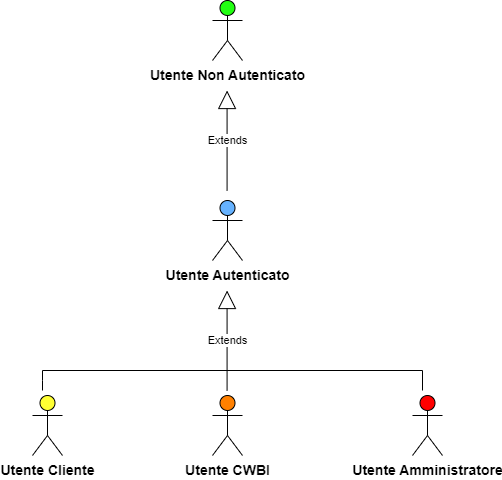
\includegraphics[width=0.9\columnwidth]{usecase/utenti-primari} 
    \caption{Gerarchia degli attori}
\end{figure}

\\
\textbf{Utente Non Autenticato}: utente che ancora non ha effettuato l'accesso alla webapp. 
\\
\textbf{Utente Autenticato}: utente che ha effetuato l'accesso.  
\\ 
\textbf{Utente Cliente}: utente autenticato con permessi di livello Cliente. Rappresenta i clienti esterni all'azienda. 
\\ 
\textbf{Utente CWBI}: utente autenticato con permessi di livello CWBI. Rappresenta i dipendenti dell'azienda CWBI. 
\\
\textbf{Utente Amministratore}: utente autenticato con permessi Amministratore. Rappresenta uno o più dipendenti CWBI che hanno la funzione di amministrare la webapp e i contenuti.  \\


\subsection{Elenco}
\subsubsection{UC01 - Autenticazione}

\begin{figure}[H]
    \centering 
    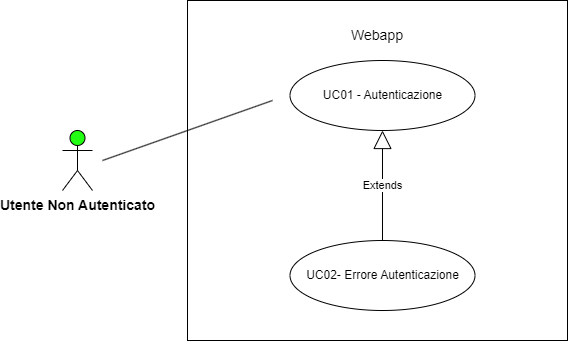
\includegraphics[width=0.9\columnwidth]{usecase/UC01}
    \caption{UC01}
\end{figure}

            \begin{table}[H]
                \centering
                \renewcommand{\arraystretch}{1.8}
                \renewcommand\tabularxcolumn[1]{m{#1}}
                \begin{tabularx}{0.9\textwidth} {
                    >{\hsize=.8\hsize\linewidth=\hsize}X
                    >{\hsize=1.2\hsize\linewidth=\hsize}X}
                    \hline
                    \textbf{Attore primario} & Utente non autenticato \\
                    \hline
                    \textbf{Precondizioni} & L'utente non è autenticato. \\
                    \hline
                    \textbf{Postcondizioni} & L'utente è autenticato. \\
                    \hline
                    \textbf{Scenario principale} & L'utente accede alla webapp \\
                    \hline
                    \textbf{Estensioni} & Se l'accesso non va a buon fine, si verifica \hyperref[UC02]{UC02}. \\
                    \hline
                \end{tabularx}
                \caption{UC01}
            \end{table}

\subsubsection{UC02 - Errore Autenticazione}

                    \begin{table}[H]
                    \centering
                    \renewcommand{\arraystretch}{1.8}
                    \renewcommand\tabularxcolumn[1]{m{#1}}
                    \begin{tabularx}{0.9\textwidth} {
                        >{\hsize=.8\hsize\linewidth=\hsize}X
                        >{\hsize=1.2\hsize\linewidth=\hsize}X}
                        \hline
                        \textbf{Attore primario} & Utente non autenticato \\
                        \hline
                        \textbf{Precondizioni} & L'utente sta tentando di autenticarsi. \\
                        \hline
                        \textbf{Postcondizioni} & L'operazione fallisce. \\
                        \hline
                        
                    \end{tabularx}
                    \caption{UC02}
                \end{table}

 			\begin{table}[H]
                	\centering
                		\renewcommand{\arraystretch}{1.8}
                		\renewcommand\tabularxcolumn[1]{m{#1}}
                		\begin{tabularx}{0.9\textwidth} {
                    >{\hsize=.8\hsize\linewidth=\hsize}X
                    >{\hsize=1.2\hsize\linewidth=\hsize}X}
                    \hline
                    \textbf{Scenario principale} &
                           \begin{enumerate}
                                \item Si verificano problemi con l'accesso alla webapp;
                                \item Viene mostrato un errore che informa l'utente del fallimento dell'operazione.
                           \end{enumerate} \\
                                            \hline
                    \end{tabularx}
                    \caption{UC02}
          	\end{table}



\subsubsection{UC03 - Registrazione Nuovo Utente}
\begin{figure}[H]
    \centering 
    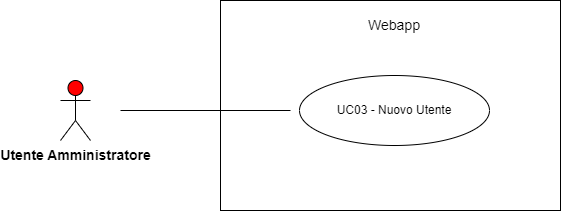
\includegraphics[width=0.9\columnwidth]{usecase/UC03}
    \caption{UC03}
\end{figure}
  \begin{table}[H]
                \centering
                \renewcommand{\arraystretch}{1.8}
                \renewcommand\tabularxcolumn[1]{m{#1}}
                \begin{tabularx}{0.9\textwidth} {
                    >{\hsize=.8\hsize\linewidth=\hsize}X
                    >{\hsize=1.2\hsize\linewidth=\hsize}X}
                    \hline
                    \textbf{Attore primario} & Utente Amministratore\\
                    \hline
             
                    \hline
                    \textbf{Precondizioni} & L'utente amministratore vuole registrare un nuovo utente\\
                    \hline
                    \textbf{Postcondizioni} & L'utente amministratore ha registrato un nuovo utente\\
                    \hline
                    \textbf{Scenario principale} & L'utente è nel modulo di registrazione utente della webapp\\
                    \hline
              
                \end{tabularx}
                \caption{UC03}
            \end{table}

\subsubsection{UC04 - Accesso Modulo Ticket}
\begin{figure}[H]
    \centering 
    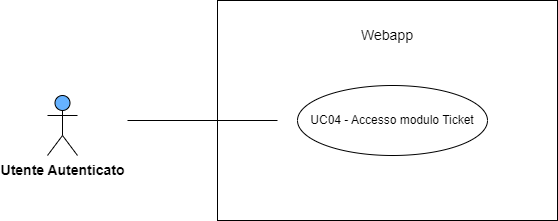
\includegraphics[width=0.9\columnwidth]{usecase/UC04}
    \caption{UC04}
\end{figure}

\begin{table}[H]
                \centering
                \renewcommand{\arraystretch}{1.8}
                \renewcommand\tabularxcolumn[1]{m{#1}}
                \begin{tabularx}{0.9\textwidth} {
                    >{\hsize=.8\hsize\linewidth=\hsize}X
                    >{\hsize=1.2\hsize\linewidth=\hsize}X}
                    \hline
                    \textbf{Attore primario} & Utente autenticato \\
                    \hline
      
                    \hline
                    \textbf{Precondizioni} & L'utente è nella webapp \\
                    \hline
                    \textbf{Postcondizioni} & L'utente è nel modulo ticket \\
                    \hline
                    \textbf{Scenario principale} & L'utente accede al modulo ticket e alle sue funzionalità \\
                    \hline
                \end{tabularx}
                \caption{UC04}
            \end{table}
            
  
\subsubsection{UC05 - Visualizza Lista Ticket}  
        
        \begin{figure}[H]
    \centering 
    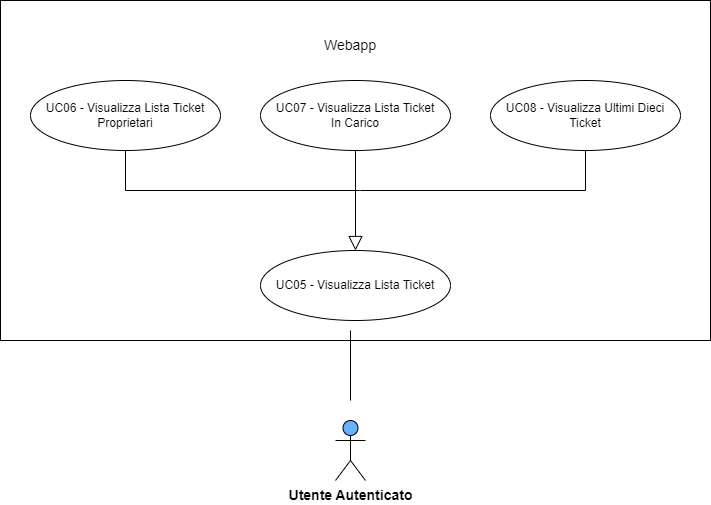
\includegraphics[width=0.8\columnwidth]{usecase/UC05_06_07}
    \caption{UC05 - UC06 - UC07 - UC08}
\end{figure}

\subsubsection{UC06 - Visualizza Lista Ticket Proprietari}  
 \begin{table}[H]
                \centering
                \renewcommand{\arraystretch}{1.8}
                \renewcommand\tabularxcolumn[1]{m{#1}}
                \begin{tabularx}{0.9\textwidth} {
                    >{\hsize=.8\hsize\linewidth=\hsize}X
                    >{\hsize=1.2\hsize\linewidth=\hsize}X}
                    \hline
                    \textbf{Attore primario} & Utente autenticato \\
                    \hline
                    \textbf{Precondizioni} & L'utente è nella pagina principale della webapp \\
                    \hline
                    \textbf{Postcondizioni} & L'utente visualizza la lista dei ticket aperti da lui. \\
                    \hline
                    \textbf{Scenario principale} & L'utente sceglie di visualizzare i ticket proprietari. \\
                    \hline
                \end{tabularx}
                \caption{UC06}
            \end{table}
     
     
\subsubsection{UC07 - Visualizza Lista Ticket In Carico}  
 \begin{table}[H]
                \centering
                \renewcommand{\arraystretch}{1.8}
                \renewcommand\tabularxcolumn[1]{m{#1}}
                \begin{tabularx}{0.9\textwidth} {
                    >{\hsize=.8\hsize\linewidth=\hsize}X
                    >{\hsize=1.2\hsize\linewidth=\hsize}X}
                    \hline
                    \textbf{Attore primario} & Utente autenticato \\
                    \hline
                    \textbf{Precondizioni} & L'utente è nella pagina di visualizzazione dei ticket. \\
                    \hline
                    \textbf{Postcondizioni} & L'utente visualizza la lista dei ticket presi in carico. \\
                    \hline
                    \textbf{Scenario principale} & L'utente sceglie di visualizzare i ticket presi in carico. \\
                    \hline
                \end{tabularx}
                \caption{UC07}
            \end{table}
            
\subsubsection{UC08 - Visualizza Lista Degli Ultimi Dieci Ticket}  
 \begin{table}[H]
                \centering
                \renewcommand{\arraystretch}{1.8}
                \renewcommand\tabularxcolumn[1]{m{#1}}
                \begin{tabularx}{0.9\textwidth} {
                    >{\hsize=.8\hsize\linewidth=\hsize}X
                    >{\hsize=1.2\hsize\linewidth=\hsize}X}
                    \hline
                    \textbf{Attore primario} & Utente autenticato \\
                    \hline
                    \textbf{Precondizioni} & L'utente è nella pagina di visualizzazione dei ticket \\
                    \hline
                    \textbf{Postcondizioni} & L'utente visualizza la lista degli ultimi dieci ticket aperti. \\
                    \hline
                    \textbf{Scenario principale} & L'utente sceglie di visualizzare gli ultimi dieci ticket aperti.\\
                    \hline
                \end{tabularx}
                \caption{UC08}
            \end{table}            
    

\subsubsection{UC05.1, UC05.2}

\begin{figure}[H]
    \centering 
    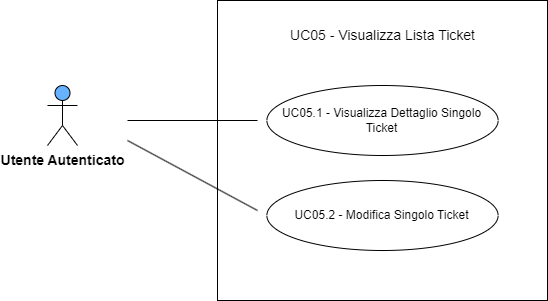
\includegraphics[width=0.9\columnwidth]{usecase/UC05_1_2}
    \caption{UC05.1 - UC05.2}
\end{figure}
\subsubsection{UC05.1}
  \begin{table}[H]
                \centering
                \renewcommand{\arraystretch}{1.8}
                \renewcommand\tabularxcolumn[1]{m{#1}}
                \begin{tabularx}{0.9\textwidth} {
                    >{\hsize=.8\hsize\linewidth=\hsize}X
                    >{\hsize=1.2\hsize\linewidth=\hsize}X}
                    \hline
                    \textbf{Attore primario} & Utente autenticato \\
                    \hline
                    \textbf{Precondizioni} & L'utente ha visualizzato la lista dei ticket \\
                    \hline
                    \textbf{Postcondizioni} & L'utente visualizza il dettaglio del ticket \\
                    \hline
                    \textbf{Scenario principale} & L'utente seleziona il bottone "Dettaglio" per visualizzare i dettagli del ticket \\
                    \hline
                  
                \end{tabularx}
                \caption{UC05.1}
            \end{table}   
   
\subsubsection{UC05.2}
  \begin{table}[H]
                \centering
                \renewcommand{\arraystretch}{1.8}
                \renewcommand\tabularxcolumn[1]{m{#1}}
                \begin{tabularx}{0.9\textwidth} {
                    >{\hsize=.8\hsize\linewidth=\hsize}X
                    >{\hsize=1.2\hsize\linewidth=\hsize}X}
                    \hline
                    \textbf{Attore primario} & Utente autenticato \\
                    \hline
                    \textbf{Precondizioni} & L'utente ha visualizzato la lista dei ticket \\
                    \hline
                    \textbf{Postcondizioni} & L'utente modifica del ticket \\
                    \hline
                    \textbf{Scenario principale} & L'utente seleziona il bottone "Modifica" per modificare il ticket \\
                    \hline
                  
                \end{tabularx}
                \caption{UC05.2}
            \end{table}   
                        
\subsubsection{UC05.1 - Dettaglio}

\begin{figure}[H]
    \centering 
    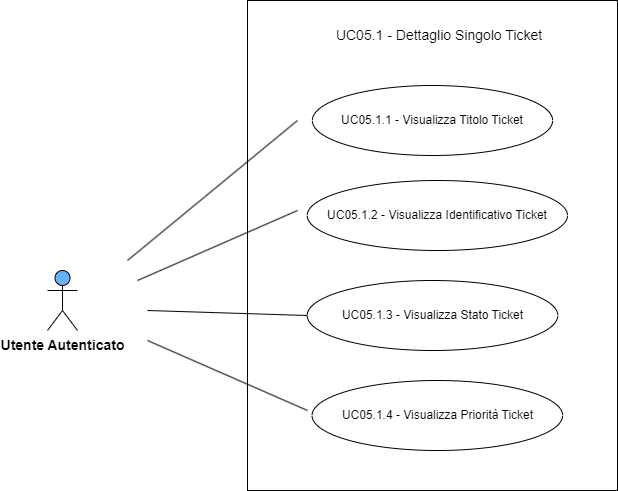
\includegraphics[width=0.8\columnwidth]{usecase/UC05_dettaglio_pt1}
    \caption{UC05.1 - Dettaglio}
\end{figure}
             \begin{figure}[H]
    \centering 
    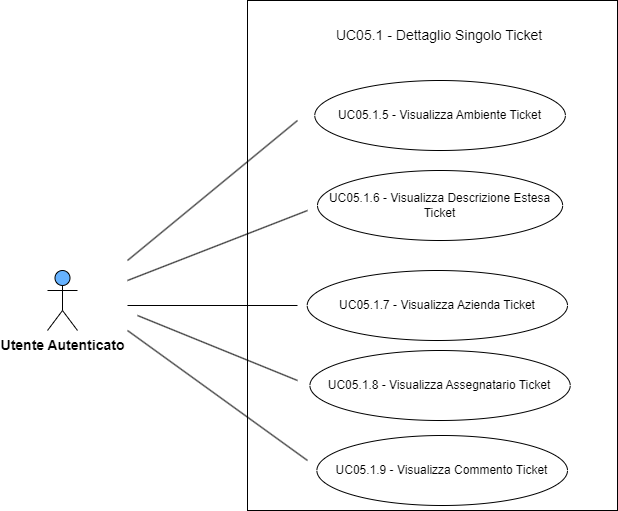
\includegraphics[width=0.8\columnwidth]{usecase/UC05_dettaglio_pt2}
\end{figure} 
        
\begin{table}[H]
                \centering
                \renewcommand{\arraystretch}{1.8}
                \renewcommand\tabularxcolumn[1]{m{#1}}
                \begin{tabularx}{0.9\textwidth} {
                    >{\hsize=.8\hsize\linewidth=\hsize}X
                    >{\hsize=1.2\hsize\linewidth=\hsize}X}
                    \hline
                    \textbf{Attore primario} & Utente autenticato \\
                    \hline
                    \textbf{Precondizioni} & L'utente ha selezionato da una lista il dettaglio di un ticket \\
                    \hline
                    \textbf{Postcondizioni} & L'utente visualizza i dettagli del ticket \\
                    \hline
                    \textbf{Scenario principale} & L'utente visualizza tutte le informazioni del ticket: titolo, descrizione, data di apertura, ecc... \\
                    \hline
                \end{tabularx}
                \caption{UC05.1 - Dettaglio}
            \end{table}  
           
\subsubsection{UC09 - Apertura Nuovo Ticket}

\begin{figure}[H]
    \centering 
    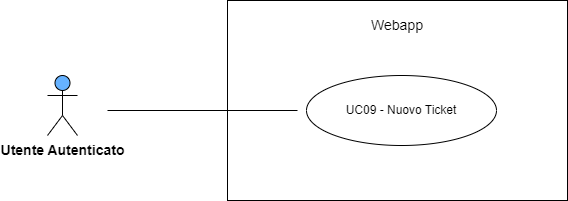
\includegraphics[width=0.7\columnwidth]{usecase/UC09}
    \caption{UC09}
\end{figure}
 

 \begin{table}[H]
                \centering
                \renewcommand{\arraystretch}{1.8}
                \renewcommand\tabularxcolumn[1]{m{#1}}
                \begin{tabularx}{0.9\textwidth} {
                    >{\hsize=.8\hsize\linewidth=\hsize}X
                    >{\hsize=1.2\hsize\linewidth=\hsize}X}
                    \hline
                    \textbf{Attore primario} & Utente autenticato \\
                    \hline
                    \textbf{Precondizioni} & L'utente crea un nuovo ticket compilando i campi: azienda, progetto, titolo, descrizione, data di scadenza, ambiente, priorità, stato, allegato. \\
                    \hline
                    \textbf{Postcondizioni} & L'utente apre un nuovo ticket, compilando tutti i campi \\
                    \hline
                    \textbf{Scenario principale} & L'utente, accedendo al modulo ticket, seleziona la creazione di un nuovo ticket \\
                    \hline
                    \textbf{Estensioni} & Se la creazione di un ticket non va a buon fine, si verifica \hyperref[UC17]{UC17}. \\

                    \hline
                \end{tabularx}
                \caption{UC09}
\end{table}

\subsubsection{UC10 - Ricerca Ticket}

\begin{figure}[H]
    \centering 
    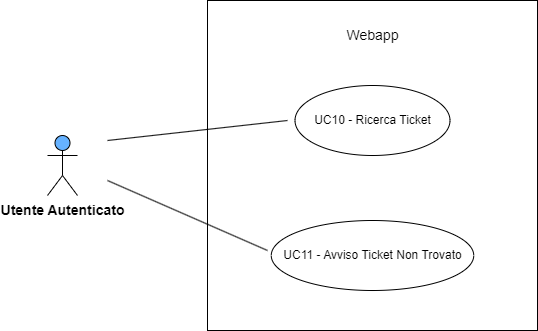
\includegraphics[width=0.9\columnwidth]{usecase/UC10_11}
    \caption{UC10 - UC11}
\end{figure}
 
\begin{table}[H]
                \centering
                \renewcommand{\arraystretch}{1.8}
                \renewcommand\tabularxcolumn[1]{m{#1}}
                \begin{tabularx}{0.9\textwidth} {
                    >{\hsize=.8\hsize\linewidth=\hsize}X
                    >{\hsize=1.2\hsize\linewidth=\hsize}X}
                    \hline
                    \textbf{Attore primario} & Utente autenticato \\
                    \hline
                    \textbf{Precondizioni} & L'utente è nella pagina di ricerca di ticket. \\
                    \hline
                    \textbf{Postcondizioni} & L'utente ha ricercato e trovato uno o più ticket. \\
                    \hline
                    \textbf{Scenario principale} & L'utente ricerca i ticket \\
                    \hline
                    \textbf{Estensioni} & Se la ricerca non dà nessun risultato, si verifica \hyperref[UC11]{UC11}. \\
                    \hline
                \end{tabularx}
                \caption{UC10 - UC11}
            \end{table}
            
\begin{figure}[H]
    \centering 
    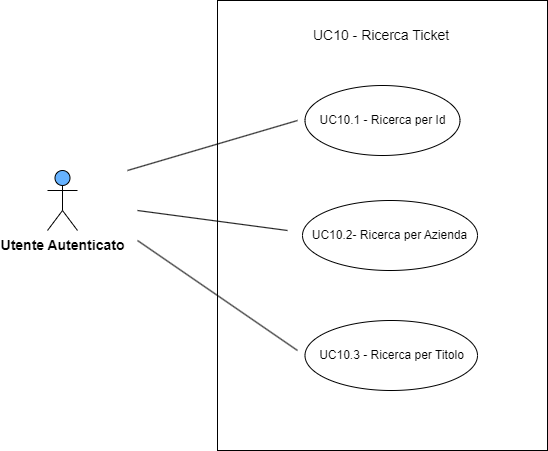
\includegraphics[width=0.7\columnwidth]{usecase/UC10_ricerca_p1}
    
\end{figure}     
\begin{figure}[H]
    \centering 
    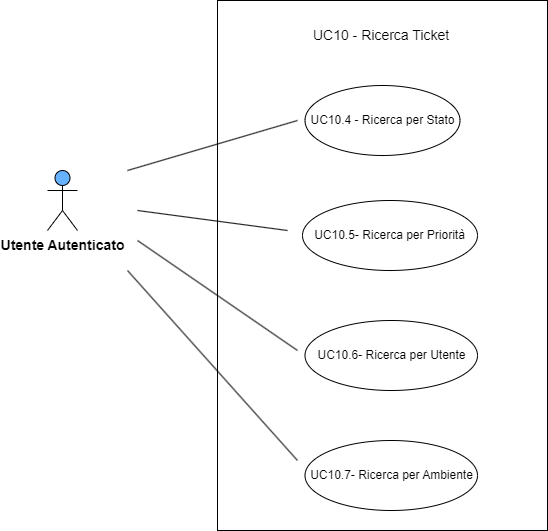
\includegraphics[width=0.7\columnwidth]{usecase/UC10_ricerca_p2}
    \caption{Filtri}
\end{figure}  
\begin{table}[H]
                \centering
                \renewcommand{\arraystretch}{1.8}
                \renewcommand\tabularxcolumn[1]{m{#1}}
                \begin{tabularx}{0.9\textwidth} {
                    >{\hsize=.8\hsize\linewidth=\hsize}X
                    >{\hsize=1.2\hsize\linewidth=\hsize}X}
                    \hline
                    \textbf{Attore primario} & Utente autenticato \\
                    \hline
                    \textbf{Precondizioni} & L'utente è nella pagina di ricerca di ticket. \\
                    \hline
                    \textbf{Postcondizioni} & L'utente ha ricercato attraverso dei filtri. \\
                    \hline
                    \textbf{Scenario principale} & L'utente seleziona i filtri con cui effettuare la ricerca. \\
                    \hline
                    
                \end{tabularx}
                \caption{UC10 - Filtri}
            \end{table}
            

    
  \subsubsection{UC11 - Ticket Non Trovato}              
 \begin{table}[H]
                \centering
                \renewcommand{\arraystretch}{1.8}
                \renewcommand\tabularxcolumn[1]{m{#1}}
                \begin{tabularx}{0.9\textwidth} {
                    >{\hsize=.8\hsize\linewidth=\hsize}X
                    >{\hsize=1.2\hsize\linewidth=\hsize}X}
                    \hline
                    \textbf{Attore primario} & Utente autenticato \\
                    \hline
                    \textbf{Precondizioni} & L'utente ha effettuato la ricerca secondo dei filtri\\
                    \hline
                    \textbf{Postcondizioni} & Viene visualizzato un avviso perché non è stato trovato nessun ticket. \\
                    \hline
                    \textbf{Scenario principale} & La ricerca non è andata a buon fine \\
                    \hline
                   
                \end{tabularx}
                \caption{UC11}
            \end{table}               
                
                
                
\subsubsection{UC12, UC13 - Download Allegato}

\begin{figure}[H]
    \centering 
    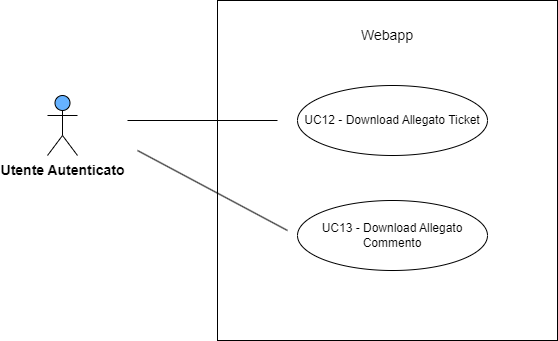
\includegraphics[width=0.9\columnwidth]{usecase/UC12_13}
    \caption{UC12 - UC13}
\end{figure}

 \subsubsection{UC12 - Download Allegato del Ticket}
 \begin{table}[H]
                \centering
                \renewcommand{\arraystretch}{1.8}
                \renewcommand\tabularxcolumn[1]{m{#1}}
                \begin{tabularx}{0.9\textwidth} {
                    >{\hsize=.8\hsize\linewidth=\hsize}X
                    >{\hsize=1.2\hsize\linewidth=\hsize}X}
                    \hline
                    \textbf{Attore primario} & Utente autenticato \\
                    \hline
                    \textbf{Precondizioni} & L'utente è nella pagina di dettaglio del Ticket\\
                    \hline
                    \textbf{Postcondizioni} & Viene scaricato l'allegato collegato al ticket. \\
                    \hline
                    \textbf{Scenario principale} & L'utente vuole scaricare l'allegato del ticket \\
                    \hline
                   
                \end{tabularx}
                \caption{UC12}
            \end{table}  
            
\subsubsection{UC13 - Download Allegato del Commento}
     \begin{table}[H]
                \centering
                \renewcommand{\arraystretch}{1.8}
                \renewcommand\tabularxcolumn[1]{m{#1}}
                \begin{tabularx}{0.9\textwidth} {
                    >{\hsize=.8\hsize\linewidth=\hsize}X
                    >{\hsize=1.2\hsize\linewidth=\hsize}X}
                    \hline
                    \textbf{Attore primario} & Utente autenticato \\
                    \hline
                    \textbf{Precondizioni} & L'utente è nella pagina di dettaglio del Ticket\\
                    \hline
                    \textbf{Postcondizioni} & Viene scaricato l'allegato collegato al commento. \\
                    \hline
                    \textbf{Scenario principale} & L'utente vuole scaricare l'allegato del commento \\
                    \hline
                \end{tabularx}
                \caption{UC13}
            \end{table}      
                 
                 
  \subsubsection{UC14 - Nuovo Commento}               
   \begin{figure}[H]
    \centering 
    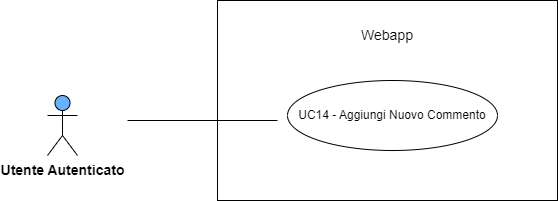
\includegraphics[width=1.1\columnwidth]{usecase/UC14}
    \caption{UC14}
\end{figure}      
        
       \begin{table}[H]
                \centering
                \renewcommand{\arraystretch}{1.8}
                \renewcommand\tabularxcolumn[1]{m{#1}}
                \begin{tabularx}{0.9\textwidth} {
                    >{\hsize=.8\hsize\linewidth=\hsize}X
                    >{\hsize=1.2\hsize\linewidth=\hsize}X}
                    \hline
                    \textbf{Attore primario} & Utente autenticato \\
                    \hline
                    \textbf{Precondizioni} & L'utente è nella pagina di dettaglio del Ticket.\\
                    \hline
                    \textbf{Postcondizioni} & L'utente ha pubblicato un commento.\\
                    \hline
                    \textbf{Scenario principale} & L'utente vuole aggiungere un commento al ticket che verrà visualizzato nella sezione "Commenti". \\
                    \hline
                    
                \end{tabularx}
                \caption{UC14}
            \end{table}
            
\begin{figure}[H]
    \centering 
    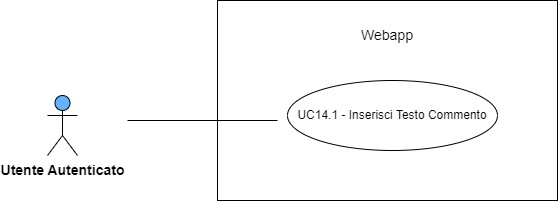
\includegraphics[width=0.7\columnwidth]{usecase/UC14_inserimentoTesto}
    \caption{UC14.1}
\end{figure}    
        
       \begin{table}[H]
                \centering
                \renewcommand{\arraystretch}{1.8}
                \renewcommand\tabularxcolumn[1]{m{#1}}
                \begin{tabularx}{0.9\textwidth} {
                    >{\hsize=.8\hsize\linewidth=\hsize}X
                    >{\hsize=1.2\hsize\linewidth=\hsize}X}
                    \hline
                    \textbf{Attore primario} & Utente autenticato \\
                    \hline
                    \textbf{Precondizioni} & L'utente è nella pagina del commento.\\
                    \hline
                    \textbf{Postcondizioni} & L'utente ha inserito il testo del commento\\
                    \hline
                    
                \end{tabularx}
                \caption{UC14.1}
            \end{table}

\subsubsection{UC15, UC16 - Eliminazione}
       
\begin{figure}[H]
    \centering 
    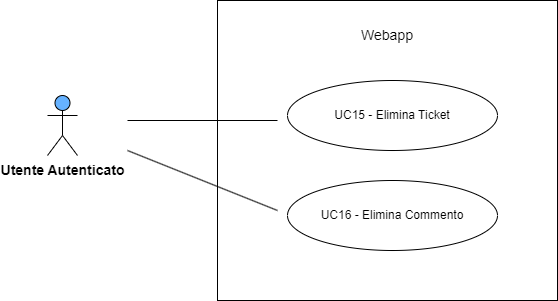
\includegraphics[width=0.7\columnwidth]{usecase/UC15_16}
    \caption{UC15 - UC16}
\end{figure}
 
\subsubsection{UC15}
 
       \begin{table}[H]
                \centering
                \renewcommand{\arraystretch}{1.8}
                \renewcommand\tabularxcolumn[1]{m{#1}}
                \begin{tabularx}{0.9\textwidth} {
                    >{\hsize=.8\hsize\linewidth=\hsize}X
                    >{\hsize=1.2\hsize\linewidth=\hsize}X}
                    \hline
                    \textbf{Attore primario} & Utente autenticato \\
                    \hline
                    \textbf{Precondizioni} & L'utente è nel modulo Ticket\\
                    \hline
                    \textbf{Postcondizioni} & L'utente ha eliminato un Ticket.\\
                    \hline
                    \textbf{Scenario principale} & L'utente vuole eliminare il ticket selezionato \\
                    \hline
                    
                \end{tabularx}
                \caption{UC15}
            \end{table}          

\subsubsection{UC16}
 
       \begin{table}[H]
                \centering
                \renewcommand{\arraystretch}{1.8}
                \renewcommand\tabularxcolumn[1]{m{#1}}
                \begin{tabularx}{0.9\textwidth} {
                    >{\hsize=.8\hsize\linewidth=\hsize}X
                    >{\hsize=1.2\hsize\linewidth=\hsize}X}
                    \hline
                    \textbf{Attore primario} & Utente autenticato \\
                    \hline
                    \textbf{Precondizioni} & L'utente è nel modulo Ticket\\
                    \hline
                    \textbf{Postcondizioni} & L'utente ha eliminato un commento.\\
                    \hline
                    \textbf{Scenario principale} & L'utente vuole eliminare un commento dalla pagina di dettaglio di un Ticket \\
                    \hline
                    
                \end{tabularx}
                \caption{UC16}
            \end{table}    

                  
\subsubsection{UC17}
            
             \begin{table}[H]
                \centering
                \renewcommand{\arraystretch}{1.8}
                \renewcommand\tabularxcolumn[1]{m{#1}}
                \begin{tabularx}{0.9\textwidth} {
                    >{\hsize=.8\hsize\linewidth=\hsize}X
                    >{\hsize=1.2\hsize\linewidth=\hsize}X}
                    \hline
                    \textbf{Attore primario} & Utente autenticato \\
                    \hline
                    \textbf{Precondizioni} & L'utente ha provato ha creare un nuovo ticket \\
                    \hline
                    \textbf{Postcondizioni} & L'utente non è riuscito a creare il nuovo ticket\\
                    \hline
                    \textbf{Scenario principale} & L'utente cerca di creare un nuovo ticket, lasciando vuoti alcuni campi\\
                   
                \end{tabularx}
                \caption{UC17}
            \end{table}
            
\newpage             
            
\section{Tracciamento dei requisiti}

Da un'attenta analisi dei requisiti e degli use case effettuata sul progetto è stata stilata la tabella che traccia i requisiti in rapporto agli use case.\\
Il requisito è così descritto:
    \begin{itemize}
    \setlength\itemsep{1em}

        \item \textbf{codice identificativo}: ogni codice 				identificativo è univoco e definito seguendo lo 					standard di codifica \textbf{R[Importanza][Tipologia]				[Codice]}  il significato delle cui voci è:
        \begin{itemize}
        \setlength\itemsep{1em}

            \item \textbf{Importanza}:
            \begin{center}
                
                \renewcommand{\arraystretch}{1.8}
                \renewcommand\tabularxcolumn[1]{m{#1}}
                \begin{tabularx}{0.85\textwidth} {
                    >{\hsize=0.1\hsize\linewidth=\hsize}X
                    >{\hsize=1.9\hsize\linewidth=\hsize}X
                }
                    \hline
                    \textbf{1} & Requisito obbligatorio: 								irrinunciabile per l'azienda e i clienti \\
                    \hline
                    \textbf{2} & Requisito desiderabile: non 							strettamente necessario ma  a valore 							aggiunto riconoscibile. \\
                    \hline
                    \textbf{3} &  Requisito opzionale: 								relativamente utile oppure contrattabile 							più avanti nel progetto. \\
                    \hline
                \end{tabularx}
                \smallskip
            \end{center}
			
            \item \textbf{Tipologia}:
            \begin{center}
                
                \renewcommand{\arraystretch}{1.5}
                \begin{tabular}{m{2em} m{10em}}
                    \hline
                    \textbf{F} & Funzionale \\
                    \hline
                    \textbf{P} & Prestazionale \\
                    \hline
                    \textbf{Q} & Qualitativo \\
                    \hline
                    \textbf{V} &  Vincolo \\
                    \hline
                \end{tabular}
                \smallskip
            \end{center}
            
            \item \textbf{Codice}: identificatore univoco del 				requisito in forma gerarchica.
        \end{itemize}

		
        \item \textbf{classificazione}: viene riportata 						l'importanza del requisito per facilitare la 						lettura;
        \item \textbf{descrizione};
        \item \textbf{fonte}: origine del requisito.
    \end{itemize}

\newpage

\subsection{Requisiti funzionali}
    
\begin{table}[!h]
\caption{Tabella del tracciamento dei requisiti funzionali}
{\renewcommand{\arraystretch}{2}
\label{tab:requisiti-funzionali}
\begin{tabularx}{\textwidth}{PXl}
\hline\hline
\textbf{Requisito} & \textbf{Descrizione}\\
\hline

R1F1 & L'utente ha la possibilità di effetuare il login\\
\hline
R1F2 & L'utente con permesso Cliente ha la possibilità di poter accedere al modulo Ticket\\
\hline
R1F3 & L'utente con permesso CWBI ha la possibilità di poter accedere al modulo Ticket\\
\hline
R1F4	 & L'utente amministratore ha la possibilità di poter accedere ai vari moduli\\
\hline
R1F5 & L'utente amministratore può registrare un nuovo utente specificandone i permessi\\
\hline
R1F6 & L'utente loggato, accedendo al modulo ticket, può visualizzare la pagina di Home\\
\hline
R1F7 & L'utente loggato, accedendo al modulo ticket, può visualizzare la pagina di Menu\\
\hline
R1F8 & L'utente loggato può visualizzare i ticket aperti da lui\\
\hline
R1F9 & L'utente loggato può visualizzare i ticket presi in carico\\
\hline
R1F10 & L'utente loggato può visualizzare gli ultimi 10 ticket aperti\\
\hline

R1F11 & L'utente loggato può creare un nuovo ticket\\
\hline
R1F11.1 & L'utente loggato, quando crea un nuovo ticket, deve selezionare l'azienda di riferimento\\
\hline
R1F11.2 & L'utente loggato, deve selezionare il progetto su cui aprire il ticket\\
\hline
R1F11.3 & L'utente loggato deve inserire il titolo del ticket\\
\hline
R1F11.4 & L'utente loggato può inserire una descrizione del ticket\\
\hline
R1F11.5 & L'utente loggato deve selezionare l'ambiente su cui aprire il ticket\\
\hline
R1F11.6 & L'utente loggato deve selezionare la priorità del ticket\\
\hline

\end{tabularx}
}
\end{table}

\begin{table}[H]
{\renewcommand{\arraystretch}{2}%}
\begin{tabularx}{\textwidth}{PXl}
\hline\hline
\textbf{Requisito} & \textbf{Descrizione}\\

\hline
R1F11.7 & L'utente loggato deve selezionare lo stato del ticket\\
\hline
R1F11.8 & L'utente loggato può inserire la data di scadenza entro il quale il ticket deve essere completato\\
\hline
R1F11.9 & L'utente loggato può inserire un allegato\\
\hline
R1F12 & Il modulo visualizza la pagina di selezione dell' azienda \\
\hline
R1F12.1 & Il modulo visualizza solo e soltanto la lista delle aziende a cui è collegato l'utente loggato \\
\hline
R1F13 & Il modulo visualizza la pagina di creazione del ticket\\
\hline
R1F13.1 & visualizza solo e soltanto i progetti collegati all'azienda selezionata\\
\hline
R1F13.2 & Il modulo fornisce 3 ambienti su cui aprire il ticket: SVIL, PROD, TEST\\
\hline
R1F13.3 & Il modulo fornisce 4 gradi di priorità (1,2,3,4)\\
\hline
R1F13.4 & Il modulo fornisce 2 stati del ticket: APERTO - CHIUSO\\
\hline
R1F13.5 & Il modulo fornisce di poter allegare file di tipo: pdf/txt\\
\hline
R1F13.6 & Il modulo fornisce la possibilità di personalizzare la descrizione del ticket\\
\hline
R1F13.7 & Il modulo fornisce di annullare la creazione di un nuovo ticket\\
\hline
R1F14 & L'utente loggato può modificare un ticket\\
\hline
R1F14.1 & L'utente loggato, in fase di modifica, deve selezionare l'utente assegnatario\\
\hline
R1F15 & L'utente loggato può eliminare un ticket\\
\hline
R1F16 & L'utente loggato può visualizzare il dettaglio del ticket\\
\hline
R1F16.1 & Il modulo visulizza il titolo del ticket\\
\hline
R1F16.2 & Il modulo visualizza l'id del ticket\\
\hline
R1F16.3 & Il modulo visualizza l'etichetta stato del ticket\\
\hline
R1F16.4 & Il modulo visualizza l'etichetta priorità del ticket\\
\hline


\end{tabularx}
}
\end{table}

\begin{table}[H]
{\renewcommand{\arraystretch}{2}
\begin{tabularx}{\textwidth}{PXl}
\hline\hline
\textbf{Requisito} & \textbf{Descrizione}\\
\hline

R1F16.5 & Il modulo visualizza l'etichetta ambiente del ticket\\
\hline
R1F16.6 & Il modulo visualizza la descrizione estesa del ticket\\
\hline
R1F16.7 & Il modulo visualizza l'azienda del ticket\\
\hline
R1F16.8 & Il modulo visualizza l'assegnatario del ticket\\
\hline
R1F16.9 & Il modulo visualizza la descrizione del ticket\\
\hline
R1F16.10 & Il modulo visualizza l'assegnatario del ticket\\
\hline
R1F17 & L'utente loggato può scaricare il file allegato al ticket\\
\hline
R1F18 & L'utente loggato può cambiare lo stato del ticket dal dettaglio\\
\hline
R1F19 & L'utente può visualizzare la lista dei commenti del ticket\\
\hline
R1F19.1 & L'utente loggato può scaricare il file allegato al singolo commento\\
\hline
R1F20 & L'utente loggato può creare un nuovo commento per un ticket\\
\hline
R1F21 & L'utente loggato può modificare un commento\\
\hline
R1F22 & L'utente loggato può eliminare un commento\\
\hline
R1F23 & L'utente loggato può allegare un file al commento\\
\hline
R1F24 & L'utente loggato può visualizzare la pagina di ricerca\\
\hline

R1F25 & L''utente loggato può ricercare i ticket\\
\hline
R1F25.1 & L'utente loggato può ricercare i ticket per identificativo\\
\hline
R1F25.2 & L'utente loggato può ricercare i ticket per azienda\\
\hline
R1F25.3 & L'utente loggato può ricercare i ticket per titolo\\
\hline
R1F25.4 & L'utente loggato può ricercare i ticket per stato\\
\hline
R1F25.5 & L'utente loggato può ricercare i ticket per priorità\\
\hline
R1F25.6 & L'utente loggato può ricercare i ticket per utente assegnato\\
\hline
R1F25.7 & L'utente loggato può ricercare i ticket per ambiente\\
\hline
\end{tabularx}
}
\end{table}

\pagebreak

\begin{table}[H]
{\renewcommand{\arraystretch}{2}
\begin{tabularx}{\textwidth}{PXl}
\hline\hline
\textbf{Requisito} & \textbf{Descrizione}\\
\hline

R1F26 & Il modulo, visualizza i bottoni di modifica su ogni riga, solo se il ticket è stato aperto dall'utente attualmente loggato \\
\hline
R1F26.1& Il modulo, per ogni riga, fornisce il bottone di dettaglio del ticket \\
\hline
R1F26.2 & Il modulo, per ogni riga, fornisce il bottone di modifica del ticket \\
\hline
R1F26.3 & Il modulo, per ogni riga, fornisce il bottone di elimina del ticket \\
\hline
R1F27 & Il modulo permette si effettuare il salvataggio del ticket\\
\hline
R1F28 & Il modulo visualizza un errore in caso il salvataggio non vada a buon fine \\
\hline
R2F28.1 & Il modulo visualizza un errore in caso il titolo sia vuoto\\
\hline
R2F28.2 & Il modulo visualizza un errore in caso la data di scadenza sia vuota\\
\hline
R2F39 & Il modulo visualizza un avviso in caso non ci siano ticket da visualizzare\\
\hline
R2F30 & Il modulo visualizza un avviso dopo l'eliminazione di un ticket\\
\hline

\end{tabularx}
}
\end{table}

\bigskip

\subsection{Requisiti di vincolo}

\begin{table}[!h]
{\renewcommand{\arraystretch}{2}
\caption{Tabella del tracciamento dei requisiti di vincolo}
\label{tab:requisiti-vincolo}
\begin{tabularx}{\textwidth}{PXl}
\hline\hline
\textbf{Requisito} & \textbf{Descrizione} \\
\hline
R1V1 & Il modulo deve limitare la modifica di un ticket\\
\hline
R1V1.1 & Il modulo permette la modifica del ticket all'utente che lo ha aperto\\
\hline
R1V1.2 & Il modulo permette la modifica del ticket all'utente amministratore\\
\hline
R1V2 & Il modulo deve limitare l'eliminazione di un ticket\\
\hline
R1V2.1 & Il modulo permette l'eliminazione del ticket all'utente che lo ha aperto\\
\hline
R1V2.2 & Il modulo permette l'eliminazione del ticket all'utente amministratore\\
\hline

R1V3 & Il modulo deve limitare la modifica di un commento\\
\hline

\end{tabularx}
}
\end{table}


\begin{table}[H]
{\renewcommand{\arraystretch}{2}
\caption{Tabella del tracciamento dei requisiti di vincolo}
\label{tab:requisiti-vincolo}
\begin{tabularx}{\textwidth}{PXl}
\hline\hline
\textbf{Requisito} & \textbf{Descrizione} \\
\hline
R1V3.1 & Il modulo permette la modifica del commento all'utente che lo ha aperto\\
\hline
R1V3.2 & Il modulo permette la modifica del commento all'utente amministratore\\
\hline
R1V4 & Il modulo deve limitare l'eliminazione di un commento\\
\hline
R1V4.1 & Il modulo permette l'eliminazione del commento all'utente che lo ha aperto\\
\hline
R1V4.2 & Il modulo permette l'eliminazione del commento all'utente amministratore\\
\hline
R1V5 & Il modulo deve essere sviluppato in Java\\
\hline
R1V6 & Il modulo integra classi preesistenti in altri moduli\\
\hline
R1V7 & Il modulo deve essere sviluppato secondo l'architettura dell'azienda\\
\hline
R1V8 & Devono essere utilizzati i framework previsti dall'azienda per lo sviluppo delle applicazioni aziendali\\
\hline

\end{tabularx}
}
\end{table}



    \chapter{Progettazione e codifica}
\label{cap:progettazione-codifica}

\intro{Il capitolo inizialmente presenta gli strumenti e le tecnologie analizzate e utilizzate per la realizzazione del prodotto. Successivamente si vede l'effettiva creazione delle classi del progetto, affiancate da una struttura preesistente fondamentale per le classi affinché il modulo funzioni e svolga la sua funzione. }\\

\section{Tecnologie e strumenti}
\label{sec:tecnologie-strumenti}

Di seguito viene data una panoramica delle tecnologie e strumenti utilizzati.

\subsection*{HTML5}
Tecnologia standard per la creazione di pagine web. Studiata attraverso il corso di Tecnologie Web.

\subsection*{CSS}
Tecnologia standard per la creazione di pagine web e il loro abbellimento. Fornisce una vasta gamma di funzionalità per la personalizzazione delle pagine. Studiata attraverso il corso di Tecnologie Web.
\subsection*{Bootstrap3/5}
Bootstrap è un framework che fornisce delle classi le quali raggruppano uno o più attributi del css, per la creazione di pagine web \textit{responsive\gls}. \\
Bootstrap è utilizzato nello stile \textit{inline} di \textit{HTML} e le sue classi vengono inserite all'interno del \textit{tag\gls} "class" di HTML di un elemento. In questo modo, specificando la classe di Boostrap che si vuole utilizzare, verrà applicato un certo stile all'elemento selezionato. Si possono concatenare più classi per un certo elemento.\\
La differenza tra le due versioni di \textit{Boostrap} 3 e 5 è nella gamma di funzionalità che offrono. La versione 5 è la più recente e molte più funzionalità di quelle precedenti, adattandosi alle nuove feature di \textit{HTML5}. \\
Ad oggi si cerca di migrare dalle versioni più vecchie a quella più recente.
\subsection*{Servlet}
Le \textit{servlet} permettono di soddisfare delle \textit{request\gls} \textit{HTTP\gls} proveniente da web. Ogni servlet viene richiamata e caricata una sola volta e poi resta in memoria per rispondere alle chiamate successive. 
\subsection*{JSP}
Le \textit{JavaServer Page} rappresentano una tecnologia fondamentale per la realizzazione di pagine web dinamiche. Infatti forniscono dei \textit{tag} speciali con i quali possono essere richiamate delle funzioni specifiche in modo da rendere la pagina dinamica. I file \textit{JSP} sono caratterizzati dell'estensione .jsp e costituiscono le vere e proprie pagine web visualizzate dall'utente; infatti sono codificate in \textit{HTML} e \textit{XML}.
\subsection*{JSTL}
\textit{JavaServer Pages Standard Tag Library} è una libreria che estende JSP offrendo nuove funzionalità per applicazioni web in \texit{JAVA EE}. 
\subsection*{Apache Struts}
\textit{Apache Struts} è un \textit{framework oper-source} che supporta lo sviluppo di applicazioni web in Java con il pattern MVC. \textit{Struts} ha il compito di organizzare le richieste del client e richiamare le funzionalità della logica di business. \\
Il framework è composto da tre elementi principali:
\begin{itemize}
\item \textit{Request Handler\gls}: viene mappato ad un URI dallo sviluppatore;
\item \textit{Response Handler\gls}: la risposta verrà passata ad un'altra risorsa che la completerà;
\item \textit{Tag}: aiutano lo sviluppatore per lo sviluppo.
\end{itemize}

\noindent
Per configurare tutti i collegamenti tra i vari elementi e le loro interazioni si utilizza il file \textit{\textbf{struts.xml}}. In questo file vengono specificati anche gli \textit{\textbf{interceptor}} per le \textit{Action} delle nostre classi. La specifica degli \textit{interceptor} è una fase importante dello sviluppo di un'applicazione web.

\subsection*{JQUERY Taconite}
\textit{JQUERY Taconite} permette di aggiornare \texit{DOM} multipli utilizzando il risultato di una singola chiamata \textit{AJAX\gls}. \\
Viene generato un \textit{XML} con le istruzioni per l'aggiornamento dei diversi \textit{DOM}.

\subsection*{Hibernate}
È un framework che permette di mappare gli oggetti del modello ad un \textit{database} relazionale. Lo sviluppatore non deve preoccuparsi di implementazione ma è \textit{Hibernate} che si occupa del collegamento al database e di eseguire le operazioni \textit{CRUD\gls}, andando a generare query e leggerne il risultato.

\subsection*{Spring}
\textit{Spring}\gls è un framework volto ad aiutare lo sviluppo di applicazioni più o meno complesse attraverso la sua architettura modulare. Spring è diviso in cinque livelli e in questo modo si possono escludere le parti non necessarie per l'applicazione.\\
L'elemento principale di \textit{Spring} è il \textit{Core Container} che ha il compito di creazione e gestione di tutti gli oggetti dell'applicazione, detti anche \textit{\textbf{beans}\gls}.
\subsection*{Wro4j}
\textit{Wro4j} è uno strumento per l'ottimizzare le risorse web e velocizzare il caricamento delle pagine. Il suo compito è quello di organizzare le risorse, come i file \textit{css} e \textit{js}, raggrupparli e farli scaricare tutti in una sola volta alla pagina web.\\
Normalmente un browser può scaricare al massimo due risorse contemporaneamente e questo limite porta ad un caricamento della pagina lento in vista di molte risorse da scaricare. \textit{Wro4j} elimina questo problema comprendendo tutte le risorse in un'unica risorsa.
\subsection*{SVNKit}
\textit{SVNKit} è uno \textit{toolkit} \textit{Open-Source} e permette l'accesso il remoto e in locale a delle \textit{repository} per le applicazioni Java. Funge anche da sistema di versionamento. 

\subsection*{Apache Maven}
\textit{Apache Maven} è uno strumento per la gestione delle dipendenze tra un progetto Java e le versioni delle librerie che servono e si occupa anche di effettuare il download di tali risorse. \\
Le relazioni tra progetto e librerie sono definite in un file \textit{XML} chiamato \textit{\textbf{pom.xml}}.

\subsection*{Apache Tomcat}
\textit{Apache Tomcat} è un server web che permette l'esecuzione di applicazioni web. Supporta le specifiche di \textit{JSP} e \textit{servlet}.\\
Esistono diverse versioni per i server \textit{Tomcat} e si può scegliere la versione che offre le funzionalità giuste per la propria applicazione.
\subsection*{DBeaver}
È un'applicazione che si occupa di gestire i database. Si possono creare nuovi database, creare tabelle, manipolare i dati, ecc...

\section{Progettazione}
\label{sec:progettazione}
La fase di progettazione era una fase cruciale per la realizzazione del progetto. Prima ancora di iniziare la progettazione del lavoro assegnato è stato importante analizzare l'ambiente già esistente, capirne il funzionamento e individuare se c'erano elementi che potevano servire al nostro scopo. \\
Una tecnica per una buona progettazione è stata concentrarsi su un elemento alla volta. Prendere in considerazione tutti gli elementi del progetto poteva sembrare più efficace e veloce, ma così facendo si avremmo perso il focus della funzione delle classi del prodotto.\\ 
Quindi l'idea era di analizzare e progettare una singola classe, controllarne il corretto funzionamento e da lì procedere ed andare avanti con lo studio per la realizzazione delle prossime classi.


\subsection{Base di Dati}
Per la progettazione della base di dati sono iniziato da un database già esistente nell'azienda e ho inserito i nuovi elementi del progetto. Poi ho eseguito un \textit{refactoring} di alcune delle tabelle preesistenti per correggerle ed adattarle a quelle nuove, senza però modificarne attributi fondamentali per le altre parti della webapp. Anche qui c'è stata allora una fase di profonda e attenta analisi per avere una base di dati consistente. 
\subsubsection*{Tabelle preesistenti}
Il progetto utilizzava tabelle preesistenti per il suo scopo. Le tabelle erano le seguenti: 
\begin{itemize}


    \item \textbf{Cliente}: questa tabella rappresentava l'entità cliente e aveva tutti gli attributi necessari per definirne lo scopo all'interno della webapp. Il cliente non era la singola persona ma bensì l'azienda a cui poi erano collegati sia i dipendenti sia i progetti richiesti da questa. Alcuni attributi presenti servono per le altre componenti della webapp;
    \item \textbf{User}: gli user erano tutte le persone coinvolte nell'azienda, interne ed esterne. Quindi la tabella comprendeva sia il personale di CWBI sia il personale delle aziende clienti;
    \item \textbf{Progetto}: questa tabella rappresentava un progetto dell'azienda. Aveva tutti gli attributi necessari ed era collegata ad un cliente. Un progetto poteva essere collegato a più aziende diverse;
    \item \textbf{ProgettoCliente}: questa tabella rappresentava la relazione tra progetto e cliente. Veniva chiamata in causa quando si doveva scegliere l'azienda e il progetto su cui si voleva aprire il ticket;
        \item \textbf{ProgettoUser}: questa tabella rappresentava la relazione tra progetto e user. Ad ogni progetto si potevano associare uno o più utenti.
\end{itemize}

\subsubsection*{Tabelle introdotte}
\begin{itemize}
	\item \textbf{Ticket}: questa tabella rappresentava l'entità ticket con tutti gli attributi che lo caratterizzavano. Aveva un collegamento all'entità ProgettoCliente in quanto il ticket era aperto per uno specifico progetto di una specifica azienda.
	
	\item \textbf{TicketItem}: questa tabella rappresentava i commenti presenti in ogni ticket. Un commento poteva avere un solo ticket di riferimento, cioè quello in cui è stato scritto.
\end{itemize}


\begin{figure}[H]
\bigskip
\bigskip
\bigskip
\bigskip
    \centering 
    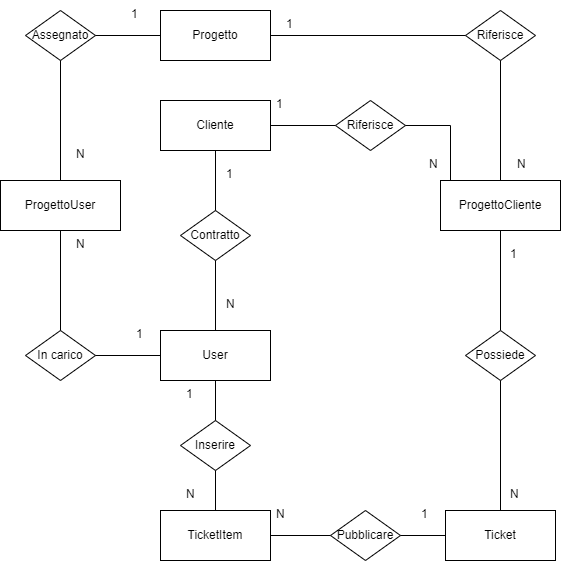
\includegraphics[width=1.1\columnwidth]{diagrammaBase} 
    \bigskip
    \caption{Base di Dati - Relazioni delle tabelle del progetto}
\end{figure}

\newpage

\begin{figure}[H]
\bigskip
\bigskip
\bigskip
\bigskip
\bigskip
    \centering 
    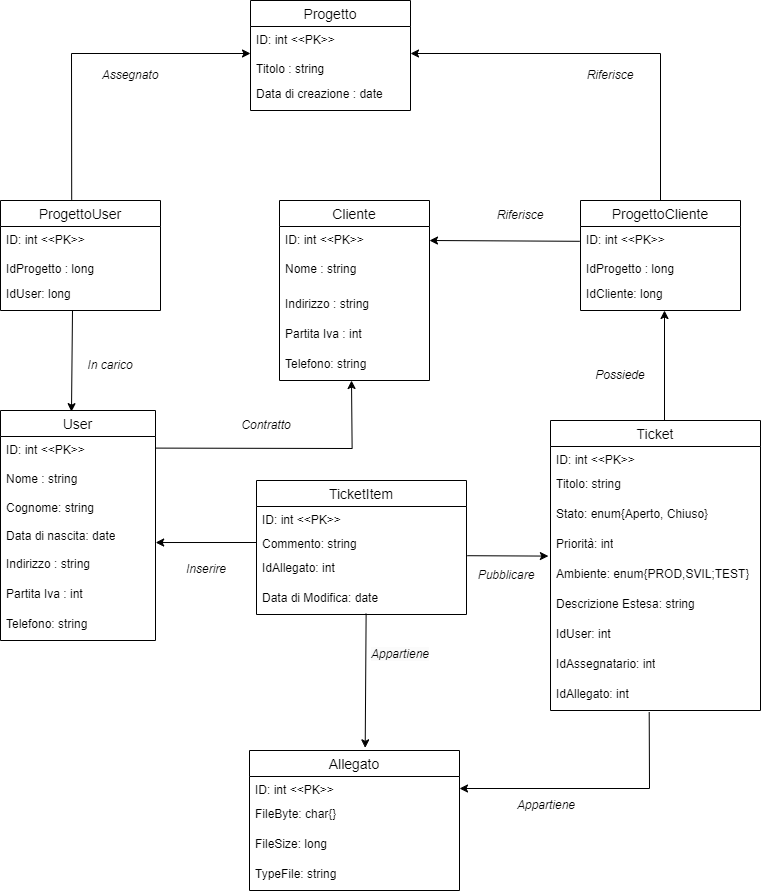
\includegraphics[width=1.1\columnwidth]{diagrammaEvoBase} 
    \bigskip
    \caption{Base di Dati - Tabelle del progetto}
\end{figure}
\newpage

\subsubsection*{Analisi delle tabelle}
            \begin{table}[H]
                \centering
                \renewcommand{\arraystretch}{1.8}
                \renewcommand\tabularxcolumn[1]{m{#1}}
                \begin{tabularx}{0.9\textwidth} {
                    >{\hsize=.8\hsize\linewidth=\hsize}X
                    >{\hsize=1.2\hsize\linewidth=\hsize}X}
                    \textbf{Cliente}\\
                    \hline
                    \textit{Id} & Identificativo univoco di ogni cliente. \\
                    \hline
                    \textit{Nome} & Nome dell'azienda.  \\
                    \hline
                    \textit{Indirizzo} & Indirizzo della sede principale dell'azienda. \\
                    \hline
                    \textit{Partita Iva} & Partita Iva dell'azienda \\
                    \hline
   	                \textit{Telefono} & Telefono dell'azienda \\
                    \hline
                \end{tabularx}
                \smallskip
                \caption{Tabella Cliente}
            \end{table}
            \smallskip
 \begin{table}[H]
                \centering
                \renewcommand{\arraystretch}{1.8}
                \renewcommand\tabularxcolumn[1]{m{#1}}
                \begin{tabularx}{0.9\textwidth} {
                    >{\hsize=.8\hsize\linewidth=\hsize}X
                    >{\hsize=1.2\hsize\linewidth=\hsize}X}
                    \textbf{ProgettoCliente}\\
                    \hline
                    \textit{Id} & Identificativo univoco di ogni ProgettoCliente. \\
                    \hline
                    \textit{IdProgetto} & Id del progetto a cui si riferisce.  \\
                    \hline
                    \textit{IdCliente} & Id dell'azienda a cui si riferisce. \\
                    \hline
                \end{tabularx}
                \smallskip
                \caption{Tabella ProgettoCliente}
            \end{table}
            \smallskip
 \begin{table}[H]
                \centering
                \renewcommand{\arraystretch}{1.8}
                \renewcommand\tabularxcolumn[1]{m{#1}}
                \begin{tabularx}{0.9\textwidth} {
                    >{\hsize=.8\hsize\linewidth=\hsize}X
                    >{\hsize=1.2\hsize\linewidth=\hsize}X}
                    \textbf{Progetto}\\
                    \hline
                    \textit{Id} & Identificativo univoco di ogni Progetto. \\
                    \hline
                    \textit{Titolo} & Titolo del progetto.  \\
                    \hline
                    \textit{Data di creazione} & Data in cui è stato aperto il progetto. \\
                    \hline
                \end{tabularx}
                \smallskip
                \caption{Tabella Progetto}
            \end{table}
            \smallskip

 \begin{table}[H]
                \centering
                \renewcommand{\arraystretch}{1.8}
                \renewcommand\tabularxcolumn[1]{m{#1}}
                \begin{tabularx}{0.9\textwidth} {
                    >{\hsize=.8\hsize\linewidth=\hsize}X
                    >{\hsize=1.2\hsize\linewidth=\hsize}X}
                    \textbf{ProgettoUser}\\
                    \hline
                    \textit{Id} & Identificativo univoco di ogni ProgettoUser. \\
                    \hline
                    \textit{IdProgetto} & Id del progetto a cui si riferisce.  \\
                    \hline
                    \textit{IdUser} & Id dell'utente a cui si riferisce. \\
                    \hline
                \end{tabularx}
                \smallskip
                \caption{Tabella ProgettoUser}
            \end{table}   
                 
    			\smallskip 
            \begin{table}[H]
                \centering
                \renewcommand{\arraystretch}{1.8}
                \renewcommand\tabularxcolumn[1]{m{#1}}
                \begin{tabularx}{0.9\textwidth} {
                    >{\hsize=.8\hsize\linewidth=\hsize}X
                    >{\hsize=1.2\hsize\linewidth=\hsize}X}
                    \textbf{User}\\
                    \hline
                    \textit{Id} & Identificativo univoco di ogni User. \\
                    \hline
                    \textit{Nome} & Nome dell'utente.  \\
                    \hline
                    \textit{Cognome} & Cognome dell'utente.  \\
                    \hline
                     \textit{Data di nascita} & Data di nascita dell'utente.  \\
                    \hline
                    \textit{indirizzo} & Indirizzo dell'utente.  \\
                    \hline
                    \textit{Partita Iva} & Partita Iva dell'utente \\
                    \hline
   	                \textit{Telefono} & Telefono dell'utente \\
                    \hline
                \end{tabularx}
                \smallskip
                \caption{Tabella User}
            \end{table}
            \smallskip 
            
 \begin{table}[H]
                \centering
                \renewcommand{\arraystretch}{1.8}
                \renewcommand\tabularxcolumn[1]{m{#1}}
                \begin{tabularx}{0.9\textwidth} {
                    >{\hsize=.8\hsize\linewidth=\hsize}X
                    >{\hsize=1.2\hsize\linewidth=\hsize}X}
                    \textbf{Ticket}\\
                    \hline
                    \textit{Id} & Identificativo univoco di ogni Ticket. \\
                    \hline
                    \textit{Titolo} & Titolo del ticket.  \\
                    \hline
                    \textit{Stato} & Stato del Ticket. \\
                    \hline
                    \textit{Priorità} & Priorità che un ticket ha. Parte da un minimo di 1, quindi poco urgente, ad un massimo di 4, urgente. \\
                    \hline            
            
                 \end{tabularx}
                \smallskip
                \caption{Tabella Ticket}
            \end{table}  
            
 \begin{table}[H]
                \centering
                \renewcommand{\arraystretch}{1.8}
                \renewcommand\tabularxcolumn[1]{m{#1}}
                \begin{tabularx}{0.9\textwidth} {
                    >{\hsize=.8\hsize\linewidth=\hsize}X
                    >{\hsize=1.2\hsize\linewidth=\hsize}X}
                    \hline
                    \textit{Ambiente} & Ambiente del Ticket. Un ticket può essere aperto in base all'ambiente in cui si sta testando l'applicazione e si trova il problema. Si hanno tre diversi ambienti: PROD, SVIL, TEST.\\
                    \hline
                    \textit{Descrizione} & Descrizione del Ticket. Utile per approfondire il problema che si è riscontrato.\\
                    \hline
                    \textit{IdUser} & Id dell'utente che ha aperto il ticket. \\
                    \hline
                    \textit{IdAssegnatario} &  Id dell'utente a cui è stato assegnato il ticket. Può essere cambiato durante il ciclo di vita del ticket. \\
                
                    \hline
                   \textit{IdAllegato} &  Id dell'allegato caricato al ticket. Può essere cambiato durante il ciclo di vita del ticket. \\
                
                    \hline
                \end{tabularx}
                \smallskip
                \caption{Tabella Ticket}
            \end{table}   
                 
    			\smallskip      

 \begin{table}[H]
                \centering
                \renewcommand{\arraystretch}{1.8}
                \renewcommand\tabularxcolumn[1]{m{#1}}
                \begin{tabularx}{0.9\textwidth} {
                    >{\hsize=.8\hsize\linewidth=\hsize}X
                    >{\hsize=1.2\hsize\linewidth=\hsize}X}
                    \textbf{TicketItem}\\
                    \hline
                     \textit{Id} & Identificativo univoco di ogni Commento. \\
                    \hline
                    \textit{Commento} & Contenuto del commento. \\
                    \hline
                    \textit{IdAllegato} & Id dell'allegato caricato al commento. \\
                    \hline
                    \textit{Data di Modifica} & Data in cui è stato modificato il ticket. \\
                    \hline
                \end{tabularx}
                \smallskip
                \caption{Tabella TicketItem}
            \end{table}
            \smallskip
            
 \begin{table}[H]
                \centering
                \renewcommand{\arraystretch}{1.8}
                \renewcommand\tabularxcolumn[1]{m{#1}}
                \begin{tabularx}{0.9\textwidth} {
                    >{\hsize=.8\hsize\linewidth=\hsize}X
                    >{\hsize=1.2\hsize\linewidth=\hsize}X}
                    \textbf{Allegato}\\
                    \hline
                    \textit{FileByte} & Contenuto del file caricato codificato in un vettore di caratteri (char[]) \\
                    \hline
                    \textit{FileSize} & Dimensione del file caricato. \\
                    \hline
                    \textit{TypeFile} & Tipo del file caricato. \\
                    \hline
                \end{tabularx}
                \smallskip
                \caption{Tabella Allegato}
            \end{table}
            
\newpage
\subsection{Architettura}
Lo sviluppo dell'applicazione è avvenuta secondo il \textit{pattern} architetturale \textbf{MVC \glsfirstoccur} (\textit{Model - View - Controller}). \\
Questo \textit{pattern} permette di dividere e rendere modulabile l'applicazione.
\begin{itemize}
\item \textbf{Model}: si occupa della gestione dei dati, del salvataggio delle risorse e della logica di business;
\item \textbf{View}: si occupa di visualizzare i dati salvati nel modello, presentandoli secondo una schema definito;
\item \textbf{Controller}: ha il compito di gestire la comunicazione tra il modello e la vista ed elaborare gli input dell'utente per poi fornire in output un determinato risultato.
\end{itemize}

\begin{figure}[H]
    \centering 
    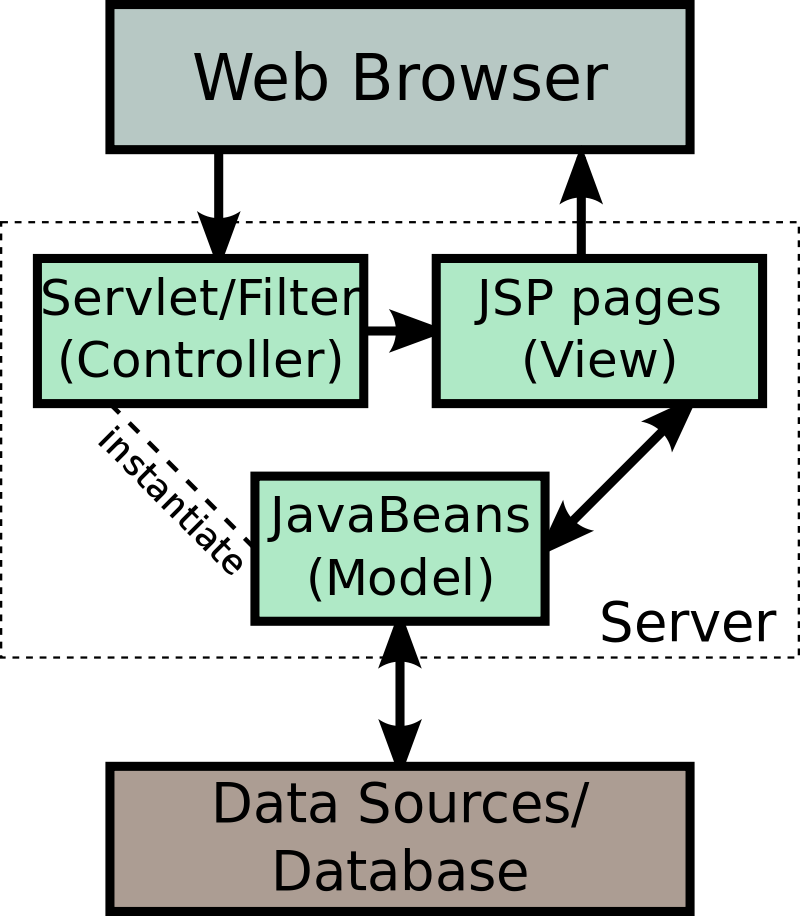
\includegraphics[width=0.4\columnwidth]{MVC} 
    \bigskip
    \caption{Schema MVC}
\end{figure}

\noindent
Utilizzare il pattern \textit{MVC} permette di avere dei \textbf{vantaggi}:
\begin{itemize}
\item \textbf{Manutenzione}: la suddivisione in componenti rende la manutenzione dell'applicazione più semplice, andando a concentrarsi sulla parte interessata;
\item \textbf{Scalabilità}: con l'aumentare delle esigenze l'applicazione richiederà degli aggiornamenti che saranno meglio integrabili;
\item \textbf{Testabilità}: senza il pattern \textit{MVC}, per eseguire il test su un parte dell'applicazione, bisognerebbe eseguire la diagnosi sul complessivo. Mentre la suddivisione in componenti permette di eseguire i test più velocemente prendendo in considerazione la parte su cui si vuole eseguirli;
\item \textbf{Separazione delle responsabilità}: ogni componente ha un compito ben preciso e non andrà a interessarsi delle parti di codice che non sono sotto la sua responsabilità.
\end{itemize}

\subsection*{Model}
Si parte da un modello preesistente e strutturato secondo gli standard aziendali. Questa parte è divisa in più livelli, ognuno dei quali ha un diverso scopo e diverse funzionalità. In generale, la struttura è illustrata come segue: 

\begin{figure}[H]
    \centering 
    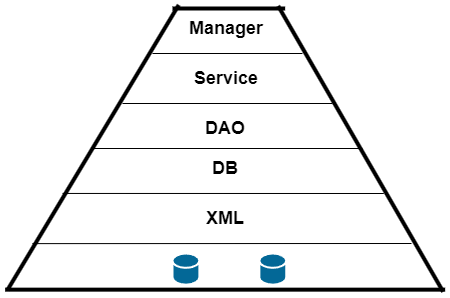
\includegraphics[width=0.6\columnwidth]{SchemaModel} 
    \bigskip
    \caption{Struttura Model CWBI}
\end{figure}

\noindent
Come detto in precedenza alcune delle classi già presenti sono utilizzate per supportare le nuove entità introdotte con il progetto. Per la codifica del nostro nuovo Model ci basiamo sulla figura \textit{5.4}, partendo dal basso e andando verso l'alto.  \\
\\
\noindent
Il primo passo per la creazione di una nuova classe è mappare i suoi attributi all'interno del file xml che conterrà la mappatura e specificherà la struttura della tabella che sarà costruita poi sul database. \\
Prendiamo come esempio la classe Ticket. Allora creeremo il file \textit{\textbf{ticket.xml}} e scriveremo la tabella \textit{ticket-a} con tutti gli attributi.\\
\\
\noindent
Dopo si comincia a codificare la classe \texttt{TicketDB.java} che rappresenta l'oggetto vero e proprio che sarà utilizzato nella  webapp. Importante specificare che gli attributi inseriti in questa classe saranno uguali agli attributi specificati nella tabella   \textit{ticket-a} nel file di mappatura. La classe sarà composta quindi dagli attributi, i costruttori e le funzioni di \textit{get} degli attributi.\\
Le nomenclatura \textit{DB} dopo il nome della classe è uno standard dell'azienda inserito per ogni nuovo modello che si introduce.
\\
\noindent
Successivamente si creano due classi: \texttt{\textbf{TicketDao}} e \texttt{\textbf{TicketDaoHibernate}}. \\
Partiamo con \textit{TicketDao} che rappresenta l'interfaccia in cui saranno presenti le firme di tutte le funzioni per la manipolazione dei dati, secondo il pattern \textit{\textbf{Dao}}: le operazioni \textit{CRUD}. \\
La classe \texttt{TicketDaoHibernate} invece è l'implementazione dell'interfaccia \texttt{TicketDao}, che implementa quindi le funzioni presenti. \\
In realtà, l'esecuzione effettiva della funzione CRUD richiesta, non avviene in \texttt{TicketDao-} \texttt{Hibernate} ma all'interno di ogni funzione implementata, viene richiamata un'altra funzione che ha lo stesso scopo di quella in cui sta venendo richiamata ma è implementata in un'altra classe \textit{Hibernate}, padre di \texttt{TicketDaoHibarnate} che 
effettuerà le operazioni classiche CRUD. \\
In generale, \texttt{TicketDaoHibarnate} implementa le funzioni dell'interfaccia a cui si riferisce, ma le operazioni CRUD vengono sempre effettuate dall'\textit{Hibernate} padre.\\

\noindent
Il prossimo passo è creare le classi service: \texttt{\textbf{TicketService}} e \texttt{\textbf{TicketServiceImpl}}.\\
La classe \texttt{TicketService} è l'interfaccia al cui interno troviamo le firme delle funzioni che la webapp consentirà di svolgere, come ad esempio la funzione di ricerca. \\
\texttt{TicketServiceImpl} invece è l'implementazione delle funzioni di \texttt{TicketService}. All'interno di ogni funzione, il dato viene manipolato e alla fine, verrà richiamata la funzione della classe \texttt{TicketDao} specifica per il contesto. 
Si può dire che all'interno dell'implementazione di una funzione \textit{service} il dato viene manipolato e personalizzato affinché, ad esempio la funzione di ricerca, ci fornisca il risultato desiderato.\\

\noindent
È importante notare che la funzione di ricerca non è una funzione \textit{CRUD} e viene implementata nel service. Infatti nella sua implementazione, questa funzione richiamerà la funzione di \textit{TicketDaoHibernate} che effettuerà la \textbf{lettura} del dato corrispondete ai parametri di ricerca.\\

\noindent
Allora tutte le funzioni all'interno delle applicazioni si riducono sempre a delle semplice funzioni \textit{\textbf{CRUD}}.\\

\noindent
L'ultima fase è creare le classi manager. Queste classi non sempre sono necessarie e fungono da supporto per le classi service. \\
Nel progetto \textbf{non} sono state codificate classi manager.

\subsection*{Controller}
Lo scopo dei \textit{controller} all'interno dell'applicazione è quello di gestire le interazioni tra la parte di \textit{front-end} (View) e la parte di \textit{back-end} (Model), oltre a gestire anche gli input degli utenti.\\

\noindent
Il \textit{controller} ha il compito di \textit{istanziare} le classi del Model, richiamarne le funzioni per avere un risultato e inviarlo poi al \textit{front-end} in modo da essere visualizzato.
All'interno dell'applicazione le classi che fungono da \textit{controller} sono marcate dall'annotazione \textit{@Controller} di Spring.\\
Un'altra annotazione Spring presente è \textit{@Autowired} che serve per indicare le dipendenze dei \textit{bean} (classi. Infatti all'interno dei controller troveremo degli oggetti \textit{Service} che saranno utilizzati per le operazioni sul Model. Quindi quando verrà istanziata il controller, anche gli oggetti all'interno di esso verranno creati.\\

\noindent
\textit{CWBI} struttura i controller in due cartelle distinte. Prendiamo come esempio la classe Ticket del modello:\\

\textbf{Cartella Form}
\begin{itemize}
\item \texttt{TicketForm}: questa classe identifica i campi di input presenti alla creazione o alla modifica di un ticket, detti appunto \textit{Form}. Quindi quando l'utente compilerà i campi, andrà a popolare gli attributi di questa classe. \\ Le caratteristiche di \texttt{TicketForm} saranno adeguate alla controparte dell'oggetto Ticket nel modello. Infatti il \textit{controller} che si occupa della creazione e della modifica, dovrà costruire l'oggetto Ticket partendo dall'oggetto TicketForm appena popolato. 

\item \texttt{TicketSearchForm}: questa classe identifica i campi di input presenti alla ricerca di un ticket. L'utente per effettuare la ricerca di un ticket potrà scegliere o compilare dei filtri , che saranno rappresentati da \texttt{TicketSearchForm}. \\
Le caratteristiche di tale classe sono redatte in base ai tipi di filtri che si vogliono fornire all'utente e devono essere adeguati per le proprietà dell'oggetto su cui si sta facendo la ricerca.

\end{itemize}
\medskip

\textbf{Cartella Action} 
\begin{itemize}
\item[] Le classi presenti in questa cartella, sono dette \textit{Action} e sono i veri e propri \textit{controller} che svolgono le varie funzioni.

\item \textttTicketAction}: come si può leggere, la classe non presenta la nomenclatura \textit{Form}. Infatti questa \textit{Action} si occupa di gestire le pagine della webapp che non hanno form al loro interno. Il dettaglio del Ticket sarà gestito da \texttt{TicketAction} in quanto non possiede nessun tipo di campo da compilare.\\
Si trovano diverse funzioni, come ad esempio la funzione di caricamento della pagina di dettaglio di un Ticket. In questa funzione viene utilizzato l'oggetto \texttt{TicketService} per richiamare la funzione di ricerca per id e trovare l'oggetto \textit{Ticket} corrispondente e stampare i dati a schermo.

\item \texttt{TicketFormAction}: questo \textit{controller} si occupa di gestire le \textit{Action} che riguardano la pagina di creazione e modifica di un \textit{Ticket} attraverso la manipolazione dell'oggetto \texttt{TicketForm}. Prendiamo come esempio la creazione di un nuovo Ticket.\\
Quando si entra nella pagina di creazione di un ticket, i campi dell'oggetto \texttt{TicketForm} sono inizializzati vuoti dall'Action \textit{input} e devono essere compilati dall'utente. Al salvataggio, viene richiamata un'altra \textit{Action} che si occupa di prendere i valori presenti nell'oggetto\texttt{TicketForm} e creare un nuovo oggetto \textit{Ticket} con i dati prelevati.\\ Alla fine, utilizzando l'oggetto\texttt{TicketService} il nuovo oggetto \textit{Ticket} viene salvato. 

\item \texttt{TicketSearchFormAction}: l'ultimo \textit{controller} è utilizzato per le pagine di ricerca di un ticket e utilizza l'oggetto \texttt{TicketSearchForm} per le proprie funzionalità. Quando si entra nella pagina di ricerca, i campi dell'oggetto\texttt{TicketSearchForm} che rappresentano i filtri di ricerca, vengono lasciati vuoti e sarà l'utente poi a riempirli. Quando si effettua la ricerca, viene richiamata la \textit{Action} di \textit{search}, dove si costruisce un nuovo oggetto \textit{Ticket} a seconda delle caratteristiche (filtri) dell'oggetto \texttt{TicketSearchForm}. \\
Viene quindi utilizzato l'oggetto \texttt{TicketService} per richiamare la funzione di ricerca che prende in input un oggetto \textit{Ticket} e confronta quale dei ticket presenti nel database ha i valori uguali a quelli del ticket passato. Vengono così trovati tutti i ticket corrispondenti ai filtri inseriti.
\end{itemize}

\subsection*{View}
L'ultimo componente dell'architettura è la \textit{\textbf{View}} che ha il compito di visualizzare i dati secondo una logica e fornire la possibilità all'utente di interagire con il modello.
\\
\noindent
Le pagine che compongono la webapp sono file \textit{jsp} che permettono di scrivere codice con standard HTML o XML, ma anche di integrare le funzionalità di Java rendendo i contenuti dinamici. \\
\newpage
\noindent
La \textbf{\textit{View}} è supportata anche da diversi \textit{framework} come \textit{Bootstrap} che fornisce delle classi per personalizzare il contenuto della pagina andando a codificare tali classi direttamente nel attributo "class" dei tag di HTML. \\
Alle pagine jsp è affiancata un'estensione detta \textit{JSTL} che mette a disposizione dei tag per la visualizzazione dei dati in modo dinamico.
\\
\noindent
Per l'interazione tra modello, controller e view entra in gioco un'ulteriore \textit{framework}, senza il quale, non sarebbe possibile il funzionamento della webapp cos' com'è stata pensata e codificata da CWBI: \textit{\textbf{Struts}}.\\

\noindent
L'utente, nell'utilizzo della webapp, interagisce con gli elementi messi a disposizione dalla \textit{View} e richiama delle specifiche \textit{Action} di controller specifici. Questa interazione è possibile grazie a \textit{Struts} che permette di associare un file jsp ad una Action di un controller, andando a configurare il file \textit{struts.xml}.

\section{Design Pattern}
I \textbf{\textit{Design Pattern}} sono soluzioni generali utilizzate per risolvere problemi ricorrenti durante lo sviluppo di un'applicazione. Esistono diversi \textit{design pattern} ed ognuno di loro ha uno scopo preciso durante la codifica del prodotto. \\
Possiamo riconoscere tre famiglie per i \textit{design pattern}:\\
\begin{itemize}
\item \textbf{Comportamentali}: definiscono le interazioni tra gli oggetti e distribuiscono le responsabilità.
\item \textbf{Creazionali}: si occupano di come creare gli oggetti
\item \textbf{Strutturali}: provvedono a definire la struttura delle classi, degli oggetti e come essi sono composti.
\end{itemize} 
\\
\noindent
L'azienda \textit{CWBI} ha applicato i seguenti \textit{design pattern} per la codifica delle loro applicazioni. Tali pattern sono anche presenti nel progetto in quanto basato su una struttura ben definita e solida.

\subsection*{Dependency Injection}
La \textit{Dependency injection} è una tecnica che si occupa di separare la creazione di un oggetto dal suo effettivo utilizzo. Quindi quando un oggetto vuole utilizzare un servizio/oggetto, non deve preoccuparsi di come questo servizio/oggetto è composto o creato in quanto li verrà \textit{iniettato} dall'esterno. Quindi le dipendenze di un oggetto con i componenti o i servizi che lo compongono sono risolte e iniettate da una classe chiamata \textbf{\textit{Injectors}}.\\
Questo \textit{pattern} porta ad avere vantaggi come il riutilizzo, la testabilità e la manutenzione del codice. 
\newpage
\subsection*{Inversion of Control}  
L' \textbf{\textit{Inversion of Control}}, detto anche \textbf{\textit{IoC}} è un design pattern molto importante ed è uno dei modi per applicare la \textit{dependency injection}.\\
Normalmente il flusso di un'applicazione è determinato dagli oggetti e quindi dal codice che la compongono. Con \textit{IoC} il controllo del flusso è affidato ad un \textit{framework} che si occuperà degli oggetti e delle loro dipendenze.\\
Un esempio di framework che applica \textit{IoC} è \textit{Spring} che introduce delle annotazioni come: \textit{@Component}, \textit{@Service}, \textit{@Repository} o \textit{@Controller}.

\subsection*{Decorator}
 \begin{figure}[H]
    \centering 
    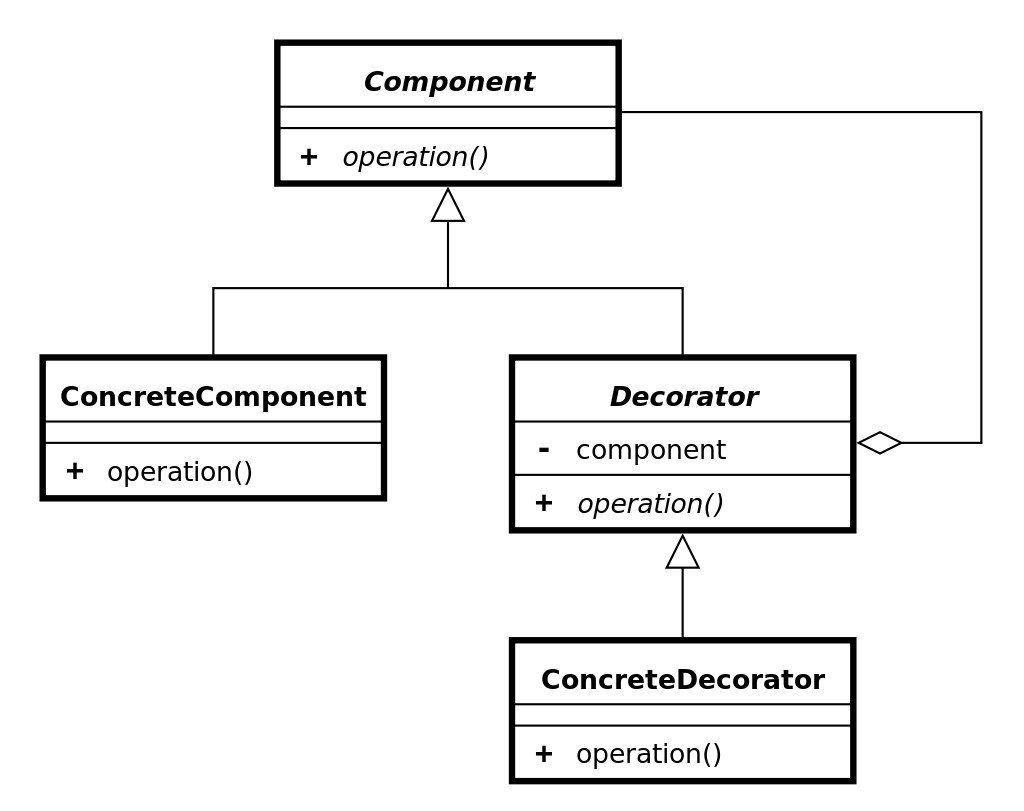
\includegraphics[width=0.6\columnwidth]{decorator} 
    \bigskip
    \caption{Pattern decorator}
\end{figure}

Il pattern \textit{\textbf{Decorator}} è un pattern strutturale che permette di introdurre nuove funzionalità e comportamenti ad un oggetto senza cambiarne la struttura. L'introduzione di questi nuovi elementi viene effettuata a \textit{run-time}.
Come si vede dalla \textit{figura 5.5} gli elementi che compongono il \textit{decorator} sono:
\begin{itemize}
\item \textbf{Component}: rappresenta l'interfaccia dell'oggetto da creare;
\item \textbf{ConcreteComponent}: è l'oggetto a cui verranno aggiunte le nuove caratteristiche;
\item \textbf{Decorator}: è l'interfaccia dei Decorator che aggiungeranno le nuove funzioni;			 
\item \textbf{ConcreteDecorator}: rappresenta gli oggetti Decorator che hanno il compito di aggiungere le nuove funzionalità al \textit{ConcreteComponent}. 
\end{itemize}
\subsection*{Data Access Object}
 \begin{figure}[H]
    \centering 
    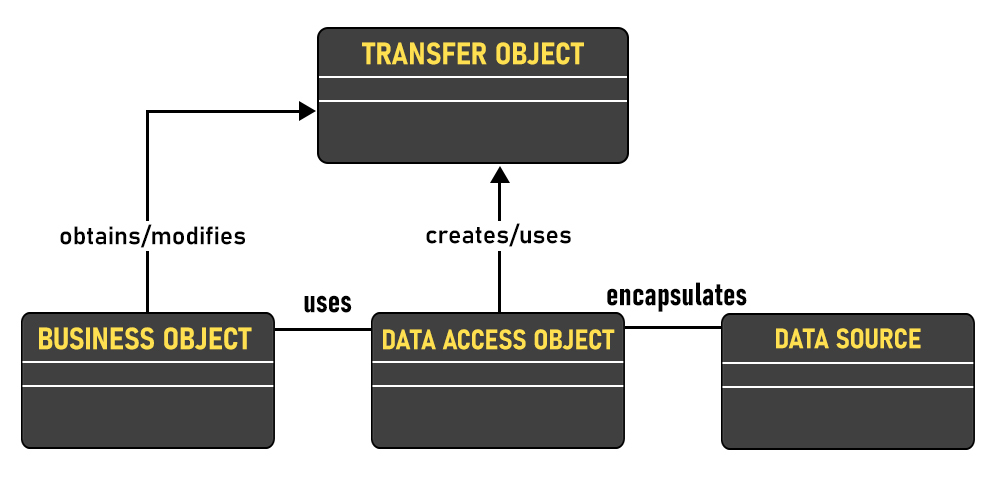
\includegraphics[width=0.7\columnwidth]{DAO} 
    \bigskip
    \caption{Pattern DAO}
\end{figure}
Il pattern \textit{\textbf{Data Access Object}}, detto anche \textit{\textbf{Dao}}, è un pattern architetturale che permette di dividere il livello di business dell'applicazione dalla fonte da cui arrivano i dati, per esempio un database. \\
Mette a disposizione un'interfaccia che mappa le operazione sui dati alle chiamate per il database. In generale, facilita l'utilizzo delle funzioni \textit{CRUD} separando i bisogni dell'applicazione dal come questi bisogni dovranno essere soddisfatti. In questo modo il livello business e il database evolveranno separatamente senza conoscere i dettagli l'uno dell'altro.

    \chapter{Verifica e validazione}
\label{cap:verifica-validazione}

Il seguente capitolo ha lo scopo di mostrare le tecniche di verifica e validazione del progetto, secondo le linee guida apprese durante il corso di Ingegneria del Software. \\
Verificare un prodotto ha l'obiettivo di controllare se l'introduzione di nuovi elementi nel codice ha generato dei problemi e se rispetta i requisiti designati. 
\\La validazione serve ad approvare il progetto qualora soddisfi tutti i requisiti imposti.

\section{Processo di Verifica}
Il processo di verifica è stato attuato durante tutto lo sviluppo del progetto per verificare le nuove funzionalità e comportamenti introdotti.\\
L'approccio all'introduzione di nuovi elementi con le relative funzioni è stato costantemente controllato da \textit{Roberto Martina}, responsabile di stage. Infatti  la tecnica più efficiente per lo sviluppo del codice era codificare una delle parti di webapp, verificare che il codice appena introdotto funzionava correttamente nel suo insieme e soltanto dopo collegarlo alle altri parti di codice già sviluppate.\\
Quindi, non si procedeva per codificare il "tutto" perché i requisiti potevano risultare non soddisfatti e c'era il rischio di perdere l'obiettivo durante lo sviluppo; ma era rigoroso procedere per passi e per ognuno verificarne la correttezza.

\subsection{Debugging}
Una delle tecniche per verificare il giusto funzionamento dell'applicazione è stato il \textit{\textbf{Debugging}}. Effettuando il debug significava controllare a \textit{run-time} come si comportava l'applicazione durante l'interazione con l'utente. Dopo aver introdotto una nuova funzione per l'applicazione si poteva effettuare il debug per verificare che la funzione introdotta funzionava nel corretto modo e non introduceva nuovi problemi per gli altri elementi già presenti. \\
Lo strumento di \textit{debug} utilizzato per verificare il progetto è quello messo a disposizione da \textbf{IDE Eclipse}. \textit{Eclipse} mette a disposizione sia il \textit{debug} del codice, ma anche il \textit{debug} per il server su cui viene eseguita la webapp.
Una feature di Eclipse è l'introduzione dei \textit{breakpoint} che permettono di verificare il codice linea per linea.\\ Inserendo un \textit{breakpoint} su una riga, 'applicazione si fermerà su quel \textit{breakpoint} durante la sua esecuzione e il programmatore con i tasti F,F10,F11,F12 potrà proseguire per ogni riga in modo da individuare la posizione esatta del possibile errore.

\begin{figure}[H]
\bigskip
    \centering 
    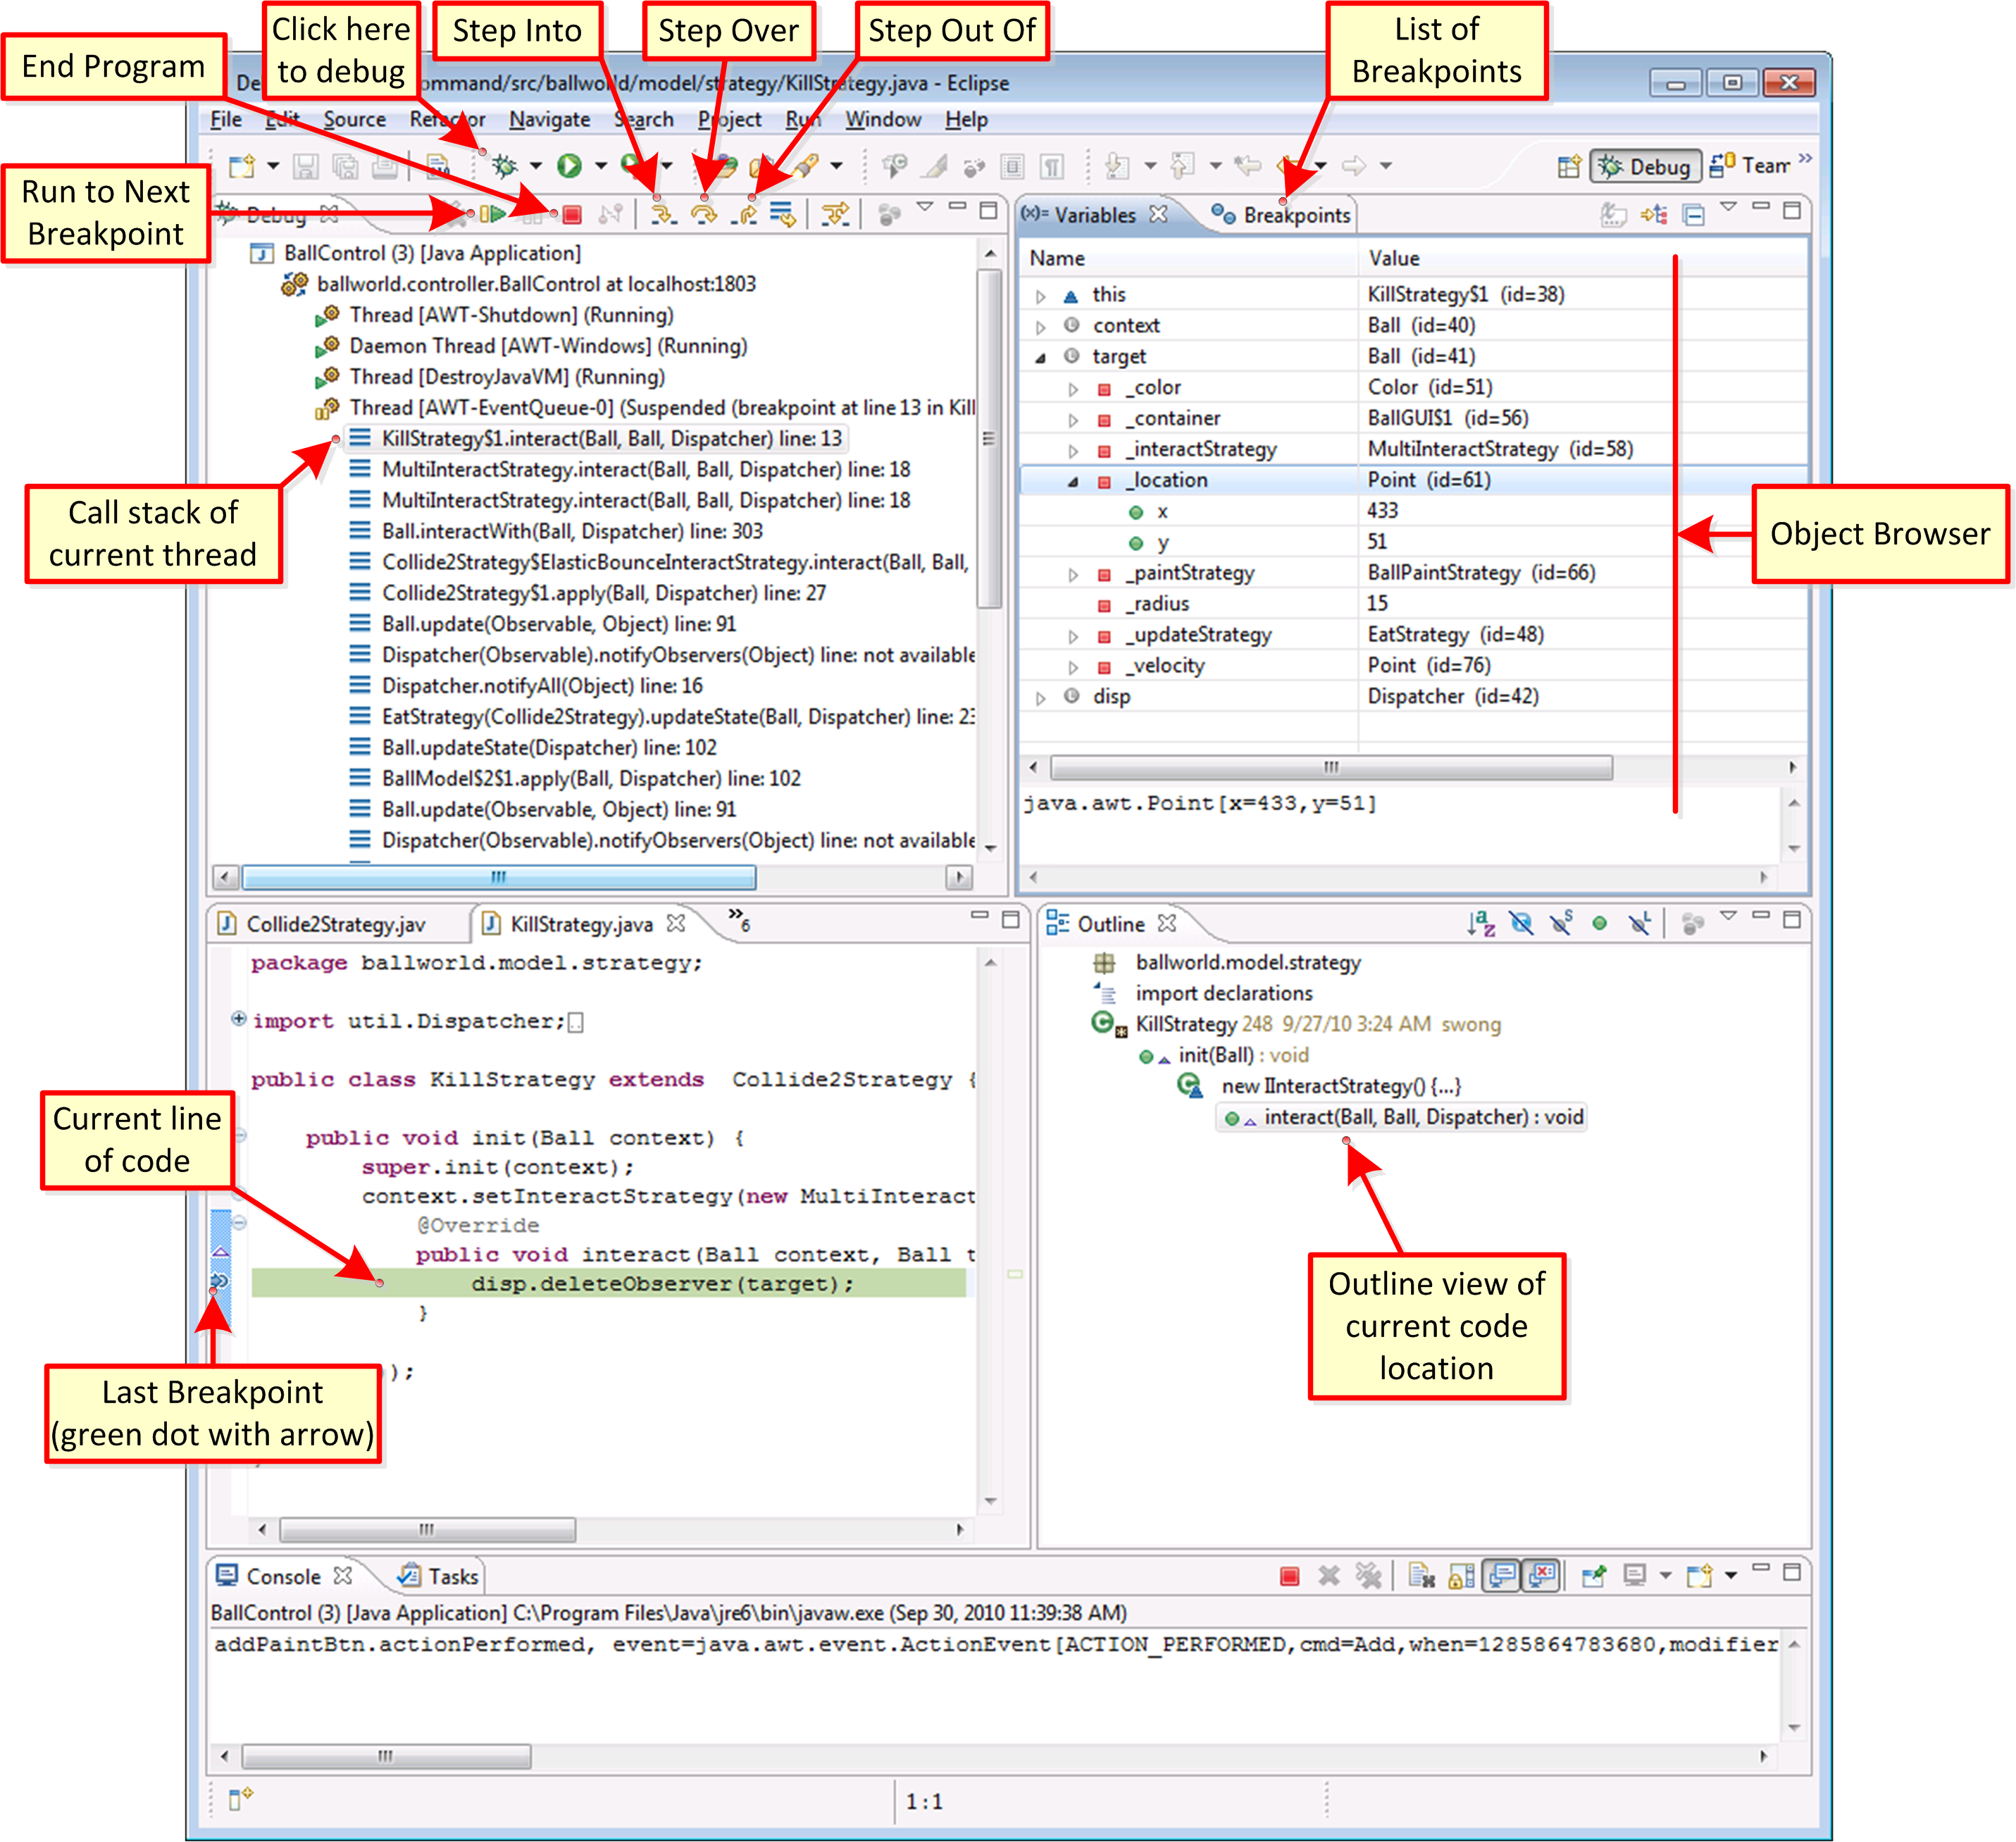
\includegraphics[width=0.7\columnwidth]{debug} 
    \bigskip
    \caption{IDE Eclipse - Debug}
\end{figure}
\bigskip
\bigskip
\section{Processo di Validazione}
Il processo di validazione è stato eseguito insieme al tutor di tirocinio \textit{Roberto Martina}. Durante gli ultimi giorni sono stati eseguiti tutti i test e confermata la validità della webapp prodotta rispetto al requisiti definiti all'inizio dello stage. \\
Oltre alla conformità ai requisiti è stato ritenuto parte fondamentale di validità del prodotto anche il rispetto dei canoni della struttura aziendale presente. \\
Il tutor ha posto quindi molta attenzione anche su questo aspetto dato che non seguire la struttura designata portava ad un uso errato dei \textit{pattern} e dei \textit{framework} utilizzati. La struttura del codice aziendale era costruita con la consapevolezza di agevolare il programmatore nella creazione di nuove classi.
    \chapter{Conclusioni}
\label{cap:conclusioni}

\section{Consuntivo finale}
La pianificazione redatta ad inizio stage sul \textit{Piano di Lavoro} ha subito delle variazione delle variazione rispetto a quante ore sono state effettivamente dedicate per ogni attività.\\ La formazione iniziale e lo studio delle tecnologie utilizzate in azienda hanno richiesto più di 40 ore, come previsto. Infatti la comprensione della struttura aziendale è stata una delle parti cruciali per iniziare lo sviluppo del progetto. Quindi non solo sono stati affrontati e appresi le nuove tecnologie e framework già presenti, ma è stato fondamentale capire come questi elementi interagiscono tra di loro nell'architettura dell'azienda. \\
Un'altra attività che ha richiesto più di quanto previsto è stata lo sviluppo della soluzione ma non per la complessità di codifica del codice, bensì per la \textit{way of working} da intraprendere. Essenziale era avere le idee chiare e procedere per passi; non immaginare fin da subito l'intero prodotto con tutte le sue parti, ma lavorare su una singola componente per volta e svilupparne le caratteristiche. 
Per le attività rimanenti le ore previste sono state più che sufficienti e quelle non utilizzate sono state dedicate alle attività già citate sopra. \\
Le 300 ore totali previste sono state quindi rispettate grazie soprattutto agli strumenti messi a disposizione dall'azienda che facilitano il lavoro rendendolo veloce ed intuitivo.

\section{Raggiungimento degli obiettivi}
Gli obiettivi definiti con il tutor \textit{Roberto Martina} ad inizio stage sono stati ampiamente raggiunti. Lo studio e la comprensione della struttura aziendale sono stati eccellenti e cruciali per il raggiungimenti degli altri obiettivi, come lo sviluppo della webapp. \\
Tutte le componenti e funzionalità previste per il modulo sviluppato sono state integrate e testate per verificarne il corretto funzionamento, così come i requisiti obbligatori raccolti nella fase di "analisi dei requisiti" sono stati soddisfatti. 
\newpage
\section{Valutazione degli strumenti utilizzati}
L'\textit{IDE} utilizzato è Eclipse, già personalmente conosciuto in una versione molto precedente a quella utilizzata e riscoperto ancora più diretto e di facile utilizzo, con la possibilità di integrare nuove componentistiche per utilizzo professionale.\\
Per la visualizzazione dell'applicazione sul browser è stato utilizzato \textit{Tomcat} che si è rivelato un applicativo perfetto per lo sviluppo di applicazioni web. Alla creazione di un server \textit{Tomcat} c'era la possibilità di scegliere tra diverse opzioni in base alla versioni di Java e dei framework presenti. Configurabile facilmente con i file \textit{jar} essenziali per il corretto funzionamento del progetto.\\
In generale gli strumenti utilizzati sono stati adeguati per lo sviluppo di un'applicazione Java e li prenderò sicuramente in considerazione anche per progetti futuri.
 
\section{Miglioramenti e future estensioni}
Il modulo della webapp sviluppato, come detto precedentemente, ha soddisfatto tutti i presupposti elaborati e concordati per lo stage con il tutor. Anche il lato utente è stato ampiamente trattato, adattandolo alle linee guida dell'azienda per quanto riguarda il \textit{front-end}.\\
Tuttavia una crescita cruciale che dovrebbe affrontare il modulo riguarda il rispetto delle norme di accessibilità attuali. Infatti la maggior parte degli elementi di \textit{front-end} non sono allineati per quanto riguarda l'accessibilità, la quale negli ultimi anni è diventata la regola fondamentale che ogni applicazione web cerca di integrare.\\
Un ulteriore miglioramento deve essere l'ottimizzazione delle interazioni tra il modulo sviluppato e quelli già presenti. L' obiettivo punta al rifacimento di alcune delle classi presenti all'interno della \textit{webapp}, in modo da avere una più solida connessione con il nuovo modulo. \\
Durante la fase di sviluppo è stata ideata una nuova feature da integrare nel progetto ma lasciata in disparte per una futura estensione del modulo. L'idea era quella di fornire all'utente un' interfaccia di messaggistica per discutere con gli altri utenti sui diversi ticket aperti in tempo reale. L'introduzione di questa funzionalità richiedeva tuttavia un' ulteriore fase di analisi dei requisiti che avrebbe portato ad uno slittamento della data di fine progetto. 

\clearpage
\mbox{}
\newpage

    \appendix
    \chapter{Appendice A}

\epigraph{Citazione}{Autore della citazione}


    \backmatter
    \printglossary[type=\acronymtype, title=Acronimi e abbreviazioni, toctitle=Acronimi e abbreviazioni]
    \printglossary[type=main, title=Glossario, toctitle=Glossario]

    \cleardoublepage
\chapter{Bibliografia}

\nocite{*}

% Print book bibliography
\printbibliography[heading=subbibliography,title={Riferimenti bibliografici},type=book]

% Print site bibliography
\printbibliography[heading=subbibliography,title={Siti web consultati},type=online]

\end{document}
